\documentclass[12pt]{article}
\usepackage{xcolor,graphicx,import,fullpage,textcomp,colortbl,array,pgfplots,lscape,todonotes,booktabs,dsfont,marvosym,ulem} \usepackage[fleqn]{amsmath}% textgreek
\usepackage{graphicx,subcaption,caption,pgfplots,amsfonts}
	\newlength\figureheight
	\newlength\figurewidth
\definecolor{grey}{gray}{0.5}
\definecolor{lightgrey}{gray}{0.8}
\usepackage[numbers]{natbib} %[numbers]
%\usepackage[papersize={85cm,30cm},left=2cm,top=2cm]{geometry}
%\usepackage[a3paper,left=2cm,top=4cm,bottom=4cm]{geometry}


%if you are annoyed of the colored boxes the hyperlinks in the pdf file uncomment this instead of the plain hyperref package above:
\usepackage[colorlinks=true, linkcolor=black, citecolor=black, urlcolor=black]{hyperref}
\usepackage{NVC} %calls the style package NVC.sty created by Loes and Evert
\usepackage{glossaries,textgreek,bm}
\usepackage{hyperref}
\usepackage[framed,numbered,autolinebreaks,useliterate]{mcode}
\usepackage[toc,page]{appendix}
\newglossary[slg]{symbolslist}{syi}{syg}{List of symbols} %Generate a list of symboles
\renewcommand*{\glspostdescription}{} %Remove the dot at the end of glossary descriptions
\makeglossaries %Activate glossary commands
\usepackage{glossaryEntries}
\usepackage{amsmath}
\numberwithin{equation}{section}
\definecolor{darkred}{rgb}{.8,0,0}
\definecolor{darkgreen}{rgb}{0,.6,0}
\newcommand{\add}[1]{\textcolor{darkgreen}{\uline{#1}}}
\newcommand{\remove}[1]{\textcolor{darkred}{\sout{#1}}}
% \Add{} and \Del{} Corrections and \Mark{}
%\usepackage[active,new,noold,marker]{xrcs}
%%%%%%%%%%%%
\newcommand{\ca}{Ca$^{\text{\scriptsize 2+}}$}
\newcommand{\ip}{IP$_{\text{\scriptsize 3}}$ }
\newcommand{\jplc}{J$_{\text{\scriptsize PLC}_{\text{\scriptsize agonist}}}$}
\newcommand{\na}{Na$^{\text{\scriptsize +}}$}
\newcommand{\pot}{K$^{\text{\scriptsize +}}$}
\newcommand{\cl}{Cl$^{\text{\scriptsize -}}$}
\newcommand{\kca}{K$_{\text{\scriptsize Ca}}$}
\linespread{2.0}%\newacronym{}{}{}

% \gls{} for normal entry
% \Gls{} for capitalised
% \glspl{} for plural
% \acrfull{} for "<full> (<abbrv>)"
% \acrlong{} for "<full>"

%makenoidxglossaries

\newacronym{smc}{SMC}{smooth muscle cell}
\newacronym{ec}{EC}{endothelial cell}
\newacronym{cicr}{CICR}{Ca$^{2+}$ induced Ca$^{2+}$ release}
\newacronym{nvc}{NVC}{neurovascular coupling}
\newacronym{ip3}{IP$_3$}{inotisol trisphosphate}
\newacronym{nvu}{NVU}{neurovascular unit}
\newacronym{sr}{SR}{sarcoplasmic reticulum}
\newacronym{er}{ER}{endoplasmic reticulum}
\newacronym{hopf}{H}{Hopf}
\newacronym{fp}{FP}{fixed point}
%\newacronym{lc}{LC}{limit cycle}
\newacronym{ode}{ODE}{ordinary differential equation}
\newacronym{pde}{PDE}{partial differential equation}
\newacronym{lpc}{LPC}{limit point cycle}
\newacronym{lp}{LP}{limit point}
\newacronym{kir}{KIR}{inward rectifying K$^+$}
\newacronym{pvs}{PVS}{perivascular space}
\newacronym{ne}{NE}{neuron}
\newacronym{sc}{SC}{synaptic cleft}
\newacronym{ac}{AC}{astrocyte}
\newacronym{bt}{BT}{Bogdanov-Takens}
\newacronym{cp}{CP}{Cusp}
\newacronym{gh}{GH}{Generalised Hopf}
\newacronym{ic}{IC}{initial condition}
\newacronym{bc}{BC}{boundary condition}
\newacronym{csd}{CSD}{cortical spreading depression}
\newacronym{mpi}{MPI}{Message Passing Interface}
\newacronym{vtk}{VTK}{Visualisation Toolkit}
\newacronym{ghk}{GHK}{Goldman Hodgkin Katz}
\newacronym{plc}{PLC}{phospholipase-C}
\newacronym{pd}{PD}{Period Doubling}
\newacronym{fhn}{FHN}{FitzHugh-Nagumo}
\newacronym{2d}{2D}{two dimensional}
\newacronym{bk}{BK}{big potassium}
\newacronym{vocc}{VOCC}{voltage operated \gls{ca} channel}
\newacronym{cbf}{CBF}{cerebral blood flow}
\newacronym{ca}{Ca$^{2+}$}{calcium}
\newacronym{pot}{K$^+$}{potassium}
\newacronym{cl}{Cl$^1$}{chlorine}
\newacronym{na}{Na$^+$}{sodium}
\newacronym{atp}{ATP}{adenosine triphosphate}
\newacronym{rhs}{RHS}{right hand side}

\newacronym{trpv}{TRPV4}{transient receptor potential vanniloid-related 4}
\newacronym{no}{NO}{nitric oxide}
\newacronym{20hete}{20-HETE}{20- hydroxyeicosatetraenoic acid}
\newacronym{eet}{EET}{epoxyeicosatrienoic acid}
\newacronym{cox}{COX}{cyclooxegenase enzymes}
\newacronym{aa}{AA}{arachidonic acid}
\newacronym{PgE2}{PgE$_2$}{prostaglandin E$_2$}
\newacronym{ecs}{ECS}{extracellular space}
\newacronym{wss}{WSS}{wall sheer stress}
\newacronym{nmda}{NMDA}{N-methyl-D-aspartate}
\newacronym{sgc}{sGC}{soluble guanylyl cyclase}
\newacronym{cgmp}{cGMP}{cyclic guanosine monophosphate}
\newacronym{mglur}{mGluR}{metabotropic glutamate receptor}

\newacronym{efs}{EFS}{electro field stimulation}
\newacronym{mlc}{MLC}{myosin light chain kinase}
\newacronym{pkc}{PKC}{protein-kinase C}
\newacronym{cpi17}{CPI-17}{myosin phosphatase inhibitor protein}

\newacronym{bold}{BOLD}{blood-oxygen-level dependent}
\newacronym{fmri}{fMRI}{functional magnetic resonance imaging}
\newacronym{cbv}{CBV}{cerebral blood volume}
\newacronym{nat}{NaT}{transient Na$^+$}

\newacronym{sodpot}{Na$^+$/K$^+$}{sodium potassium}
\newacronym{nnos}{nNOS}{neuronal \gls{no} synthase}
\newacronym{enos}{eNOS}{endothelial \gls{no} synthase}
\newacronym{cmro2}{CMRO$_2$}{cerebral metabolic rate of oxygen}
\newacronym{hbo}{HbO}{oxyhemoglobin}
\newacronym{hbr}{HbR}{deoxyhemoglobin}
\newacronym{hbt}{HbT}{total hemoglobin}
\newacronym{mtt}{MTT}{mean transit time}
\newacronym{ltp}{LTP}{long term potentiation}
\newacronym{epsp}{EPSP}{excitatory postsynaptic potential}
\newacronym{ipsp}{IPSP}{inhibitory postsynaptic potential}
\newacronym{lc}{LC}{locus coeruleus}
\newacronym{lcna}{LC-NA}{noradrenalin locus coeruleus}
\newcommand{\psec}{s$^{-1}$\xspace}
\begin{document}
\title{Analysing High-Dimensional Neuroscience Models: Neurovascular Coupling. }
\author{ Tim David$^{1}$, Pierre Gremaud$^{2}$, Joey Hart$^{2}$\\
\textit{1.Department of Mechanical Engineering,} \\
\textit{University of Canterbury, New Zealand}\\
\textit{2.Department of Mathematics,}\\
\textit{North Carolina State University, Raleigh, NC}\\
}
\maketitle
\thispagestyle{empty}

%\newpage
%\textbf{BlueFern Supercomputing Unit, University of Canterbury, New Zealand}
\begin{abstract}
abstract here 
\end{abstract}
%\listoftodos
%\tableofcontents
%\newpage

\section{Introduction}\label{sec:intro}
Over the past 20 years, the use of computational models to describe physiological phenomena has grown spectacularly. This growth has provided significant advantages to the experimental community in that it can furnish results of \textit{in silico} experiments which are either ethically or physically impossible in the laboratory. However, these models have also increased in complexity with a concomitant increase in the associated number of parameters (for a variety of reasons, most notably the requirement that the models should possess complex cellular functions which are thought \textit{but not necessarily proven} to be important). These parameters, in defining the relevant phenomenon, more often than not come from a plethora of animal experiments whose relationship to the human physiology is weak.  In addition, experimental results in the public domain provide very little information on the errors in these measurements. 

Even simple physiological models tend to be  highly non-linear; their range of applicability and reliability can only be assessed  through careful analysis. For large complex systems, the sensitivity of quantities of interest to model parameters is a priori unclear. Herein lies one of the difficulties of modeling: what effect do uncertainties in parameters determined from experiment have on the output of a non-linear numerical model? Because of both model complexity and high dimensionality, sensitivity analysis is  computationally demanding and may require several ad hoc steps--such as screening (reducing the parameter dimension). Importantly, in analysing  sensitivities, we can learn significant facts about the physiology of the system which would have stayed hidden under the premise of simply producing results. 
From a purely physiological perspective, an understanding of the dominant cellular mechanisms resulting in cerebral tissue perfusion after neuronal stimulation would be of particular and important interest. 

In the above context, we investigate the sensitivity of  the \gls{nvc} response (see Section~\ref{sec:model}), which has a large parameter dimension where most (if not all) of the parameter values come from non-human experiment  with an inherent (unknown) error. We denote by $\mathbf y = (y_1, \dots, y_N)$  the {\sl state variables} of the model and by $\boldsymbol{\theta} = (\theta_1, \dots, \theta_P)$ the {\sl uncertain parameters} of the model. The evolution of the state variables is governed by a system of ordinary differential equations (ODEs) 
\begin{eqnarray}
\frac {d\boldsymbol{y}}{dt} = \mathbf{f}(\mathbf{y}, \boldsymbol{\theta}), \label{caboodle}
\end{eqnarray}
where $\mathbf{f}$ is a known function of its arguments. Equation (\ref{caboodle}) is completed with a set of initial conditions $\boldsymbol{y}(0) = \boldsymbol{y}_0$;  here, we simply take $\boldsymbol{y}_0$ as the  equilibrium solution at the parameters' nominal values, i.e., $\mathbf f(  \mathbf{y}_0, \bar{\boldsymbol{\theta}}) = 0$, where $ \bar{\boldsymbol{\theta}} = (\bar\theta_1, \dots, \bar\theta_P)$ denotes the expected values of the parameters. The supplementary material contains code and the expected values of parameters, further information can be found in \cite{Dormanns2015a}.

Based on physiological considerations, we examine three quantities of interest (QoI), see Section~\ref{sec:model}.  Let $q$ be one of our three  QoIs; while determined from the state variables, i.e., from $\mathbf y$, $q$ is  ultimately a function of the parameters alone (and possibly time), i.e.
\begin{eqnarray}
q = g(\boldsymbol{\theta}). \label{qoi}
\end{eqnarray}
The overall goal of our numerical study is to determine  which of the uncertain parameters $\theta_1, \dots, \theta_P$  are the most/least influential for each QoI. There is a substantial amount of research currently being done in applied mathematics and statistics in the corresponding field of Global Sensitivity Analysis  (GSA). How to meaningfully define ``influential" or ``non-influential" and  how to develop methods applicable to high-dimensional problems are two significant challenges of the field \cite{corvar,timegsa,stogsa,iooss,owen,saltelli}. 



The present \gls{nvc} model contains $N=67$ state variables and $P= 160$ uncertain parameters.
The complexity of the model and large parameter space dimension preclude a direct application of GSA tools. Part of our contribution in this paper is to show how to meaningfully reduce the dimension of the original problem to make it amenable to standard GSA methods


  
\section{Methodology}\label{sec:meth}

At an abstract level, our analysis may be described in a four step process: (i) define a probability distribution for $\theta$ which models its uncertainty, (ii) draw samples from this distribution, (iii) evaluate the model for each of these parameter samples, (iv) use these model evaluations to infer its sensitivity to each parameter. Subsection~\ref{sec:param_dist_fit} describes our approach for step (i). Step (ii) is easily executed using standard methods. The computational bottleneck for our analysis is the model evaluations in step (iii). While relatively large and stiff, the ODE system (\ref{caboodle}) can be  solved with standard tools and methods, here through the MATLAB routine ode15s with relative and absolute tolerances of $10^{-4}$. The evaluation of the above QoIs themselves from the ODE solutions is straightforward and can be done at low cost. Inferring the sensitivities may be done in a plurality of ways. Because of the parameter dimension and computational cost of model evaluations, we adopt a multi-phased procedure of screening, surrogate modeling, and global sensitivity analysis, described in Subsections~\ref{sec:screen}, ~\ref{sec:surrogate}, and ~\ref{sec:gsa} respectively. We summarize our method in Subsection~\ref{sec:summary}.

\subsection{Parameter Distribution Fitting}
\label{sec:param_dist_fit}

Describing the uncertainty attached to the parameter vector $\boldsymbol{\theta}$ is an important and delicate {\sl modeling assumption}. Here, we give each $\theta_i$, $i=1,\dots, 160$, a nominal value $\bar \theta_i$ and assume each parameter to be independent and uniformly distributed over the interval $[0.9\, \bar\theta_i, 1.1 \,\bar\theta_i]$, i.e., within $\pm 10\%$ of the nominal value. Larger intervals where considered for the parameters. For the NVU model under consideration, increasing the width of the interval resulted in many samples for which the solution exhibited atypical or non-physical behavior, or in some cases ode15s was unable to solve the system. Our choice of $\pm 10\%$ uncertainty is considered a reasonable compromise between accounting for uncertainty and ensuring computational feasibility. 
	
Our assumption of parameter independence is incorrect. In fact, ode15s is unable to solve the system for most samples drawn under this assumption. The parameter dependencies, which are unknown a priori, are discovered through a computational procedure akin to Approximate Bayesian Computation \cite{abc}. Our approach, described below, is computationally intractable when applied to the NVU model under consideration. We simplify the model by removing the stimulus, i.e. modeling the steady state behavior of the system. A collection of $S$ samples, $\boldsymbol{\theta}^k$, $k=1,2,\dots,S$, are drawn from our initial distribution (assuming independence) and the ODE system is solved for each parameter sample. The collection of solutions are post-processed to partition the samples $\{\boldsymbol{\theta}^k\}_{k=1}^S$ into two subsets $\{\boldsymbol{\theta}^{a_k}\}_{k=1}^{S_a}$ and $\{\boldsymbol{\theta}^{r_k}\}_{k=1}^{S_r}$, where $a_k$, $k=1,2,\dots,S_a$ denotes the samples where the steady state solution exhibited normal behavior and $r_k$, $k=1,2,\dots,S_r$ denotes the samples where it does not. We reject the samples $\{\boldsymbol{\theta}^{r_k}\}_{k=1}^{S_r}$ and fit a distribution to the accepted samples $\{\boldsymbol{\theta}^{a_k}\}_{k=1}^{S_a}$ using standard statistical methods. This new distribution is sampled $S$ times,  the ODE system is solved for each sample, and the results are post-processed into accepted and rejected samples again. We continue this process iterative until satisfactory convergence of the fitted distribution.

\subsection{Screening}
\label{sec:screen}
Having determined a parameter distribution, we evaluate the QoI $q=g(\boldsymbol{\theta})$ at $M$ different samples, denote them $\boldsymbol{\theta}^k$, $k=1,2,\dots,M$.
We fit a {\sl linear model} to the QoI under study
\begin{eqnarray}
g(\boldsymbol\theta^k) = g(\theta_1^k, \dots, \theta_P^k) \approx \beta_0 + \sum\limits_{j=1}^{160} \beta_j \theta_j^k, \quad k=1, \dots, M. \label{lr}
\end{eqnarray}
This approach yields a crude (but highly efficient here) sensitivity analysis of the model with respect to the $\theta_j$'s, $j=1,\dots, 160$. We assign a preliminary importance measure to each $\theta_j$ by computing for each of them the relative size of their coefficient in the above linear approximation, i.e.
\begin{eqnarray*}
L_j = \frac{\vert \beta_j \vert}{\sum\limits_{\ell=1}^{160} \vert \beta_\ell \vert}, \qquad j=1,\dots,160.
\end{eqnarray*}
To obtain a model with a more manageable size, we reduce the parameter space to only the $\theta_j$'s for which $L_j>0.01$. We denote these $r$ parameters $\{ \theta_{j_i}\}_{i=1}^r$. The rest of the parameters are regarded as non-influential and set to their nominal values since, even though they are uncertain, their specific values (within the given range) have little bearing of the considered QoI. In other words, we consider the approximation 
\begin{eqnarray}
g(\theta_1, \dots, \theta_{160}) \approx h(\theta_{j_1}, \dots, \theta_{j_r}), \label{reddim}
\end{eqnarray}
where $h$ is obtained from $g$ by treating the non-influential parameters as latent. In Section~\ref{sec:results}, this reduction yields around 15-20 parameters instead of the original 160. We denote by $\hat{\boldsymbol{\theta}}$ the reduced parameter vector. 

\subsection{Surrogate model}
\label{sec:surrogate}
For any of the three considered QoIs, our information on the function $h$ defined (\ref{reddim}) consists of the set of sampled values $\{ h(\theta_{j_1}^k, \dots, \theta_{j_r}^k)\}$, $k=1, \dots, M$.  To facilitate the use of standard GSA tools, which may require derivatives or variance estimations, it is both convenient and computationally advantageous to construct an approximating function, i.e., a surrogate model. 
We use a sparse Polynomial Chaos (PC) surrogate. This amounts to introducing a polynomial approximation of $h$ of the type
\begin{eqnarray}
h(\hat{\boldsymbol{\theta}}) \approx H(\hat{\boldsymbol{\theta}}) \equiv \sum_{\boldsymbol{\alpha}} c_{\boldsymbol{\alpha}} \psi_{\boldsymbol{\alpha}}(\hat{\boldsymbol{\theta}}) \label{pce}
\end{eqnarray}
where the $\psi_{\boldsymbol{\alpha}}$'s are multivariate polynomials which are orthogonal with respect to the probability distribution function (PDF) $p_{\boldsymbol{\theta}}$ of $\boldsymbol{\theta}$, i.e.
\begin{eqnarray}
\int \psi_{\boldsymbol{\alpha}}(\mathbf x) \psi_{\boldsymbol{\beta}}(\mathbf x)\, p_{\boldsymbol{\theta}}(\mathbf x) \, d\mathbf{x} = \delta _{\boldsymbol{\alpha},\boldsymbol{\beta}} \label{ortho}
\end{eqnarray}
where $\boldsymbol{\alpha}$ and $\boldsymbol{\beta}$ are multi-indices and $\delta _{\boldsymbol{\alpha},\boldsymbol{\beta}}$ is the generalized Kronecker symbol. The coefficients are computed through least-squares minimization, see the Appendix for additional discussion. All surrogate models are validated using 10-fold cross validation.

Polynomial Chaos is by now a well documented method. We use the \textit{UQLab} implementation for the results below and refer the reader to its manual \cite{uqlab} for more details.


\subsection{Global sensitivity analysis} 
\label{sec:gsa}
We use variance based GSA to assess the relative importance of the input parameters of $H$ in (\ref{pce}). In their simplest form,  the total Sobol' indices \cite{saltellitotalindex} apportion to uncertain parameters, or sets thereof, their relative contribution to the variance of the output. Indeed, thanks to the law of total variance, we can decompose the variance of $q = H(\hat{\boldsymbol{\theta}})$ as follows
\begin{eqnarray}
\operatorname{var}(q) = \operatorname{var}(\mathbb E[q|\hat{\boldsymbol{\theta}}_{\sim i}]) + \mathbb E[\operatorname{var}(q|\hat{\boldsymbol{\theta}}_{\sim i})], \label{ltv}
\end{eqnarray}
where $\hat{\boldsymbol{\theta}}_{\sim i}$ denotes all the parameters in $\hat{\boldsymbol{\theta}}$ except $\hat{\boldsymbol{\theta}}_i$. If we assume now that all the input parameters of $H$ are known with certainty, i.e,, if $\hat{\boldsymbol{\theta}}_{\sim i}$ is known, then the remaining variance of $q$ is simply given by 
\begin{eqnarray*}
\operatorname{var}(q) - \operatorname{var}(\mathbb E[q|\hat{\boldsymbol{\theta}}_{\sim i}]) = \mathbb E[\operatorname{var}(q|\hat{\boldsymbol{\theta}}_{\sim i})]. 
\end{eqnarray*}
This latter expression is thus a natural way of measuring how influential $\hat{\boldsymbol{\theta}}_i$ is; the corresponding total Sobol' index $S_{T_i}$ is but a scaled version of this
\begin{eqnarray}
S_{T_i} = \frac{\mathbb E[\operatorname{var}(q|\hat{\boldsymbol{\theta}}_{\sim i})]}{\operatorname{var}(q) }. \label{sobol}
\end{eqnarray}
The relevance of this basic definition can be extended to time dependent QoIs \cite{timegsa}, stochastic QoIs \cite{stogsa} or correlated parameters \cite{corvar}.


\subsection{Summary of the Method}
\label{sec:summary}
Algorithm~\ref{algo} provides a summary of the method. 

\begin{algorithm}
\caption{overall numerical approach}\label{algo}
\begin{algorithmic}[1]
\While{parameter distribution has not converged}
\For{$k=1:S$} \Comment{sampling}
\State sample parameter distribution  $\longrightarrow \boldsymbol{\theta}^k$; solve (\ref{caboodle}) (without stimulus) $\longrightarrow \mathbf y^k$
\EndFor
\State partition the parameter samples into accepted and rejected samples
\State fit a new distribution to the accepted samples \Comment{see \S~\ref{sec:param_dist_fit}}
\EndWhile
\For{$k=1:M$} \Comment{sampling (final distribution)}
\State sample parameter distribution  $\longrightarrow \boldsymbol{\theta}^k$; solve (\ref{caboodle}) (with stimulus) $\longrightarrow \mathbf y^k$
\EndFor
\For{each QoI $q$}
\State solve the least-squares problem (\ref{lr}) \Comment{linear approximation}
\State identify the influential parameter vector $\hat{\boldsymbol\theta} =   (\theta_{j_1}, \dots, \theta_{j_r})$  \Comment{screening}
\State solve the least-squares problem  (\ref{pce}) for the polynomial  approximation $H$ \Comment{surrogate model}
\State compute total Sobol' indices (\ref{sobol}) for the surrogate model $H$ \Comment{global sensitivity analysis}
\EndFor
\end{algorithmic}
\end{algorithm}






\section{Numerical results}
\label{sec:results}

\subsection{Parameter distribution}
\label{sec:param_sampling}

Applying the methodology described in Section~\ref{sec:param_dist_fit}, $S=919$ parameter samples are drawn and \eqref{caboodle} is solved for each sample with no stimulus applied. Of these 919 runs, 670 of them fail due to ode15s terminating prematurely because its time steps became too small. The remaining 249 yields 139 solutions for which the radius reaches a stable steady state (at least for the duration of the time integration) and 110 solutions for which the radius reaches a steady state but subsequently because transient. The left panel of Figure~\ref{steady_states} displays four representative solutions for the radius; the red curves remain in steady state for the duration of our time integration whereas the black curves revert into a transit regime after some time in or near steady state. The right panel of Figure~\ref{steady_states} displays the samples for two parameters (in the buffer equation) which are found to be highly influential in determining the behavior of the solution. A blue \textcolor{blue}{*} indicates a sample where the solver terminated prematurely, a yellow \textcolor{yellow}{$\Diamond$} indicates a sample where an unstable steady state was observed, a red \textcolor{red}{$\circ$} indicates a sample where the solution remained in steady state. A strong correlation determining the behavior of the solution is observed. The two parameters in question, denoted by ($p_1,p_2$), occur in the buffer equation
\begin{eqnarray}\label{eqn:buff}
[K^+]_e+B \quad\begin{array}{c}
f_f \\ 
 \rightleftharpoons \\
f_r
\end{array} 
[K^+]_b \nonumber \\
\frac{d[K^+]_b}{dt}=f_f[K^+]_e(b_0-[K^+]_b)-f_r[K^+]_b \nonumber \\
f_f=\frac{f_r}{1+exp(\frac{-[K^+]_e+p_1}{p_2})}
\end{eqnarray}
The parameters $p_1$ and $p_2$ have values 5.5 and 1.09, representing a shift and scaling in the rate constant respectively. 
\begin{figure}[h]
\centering
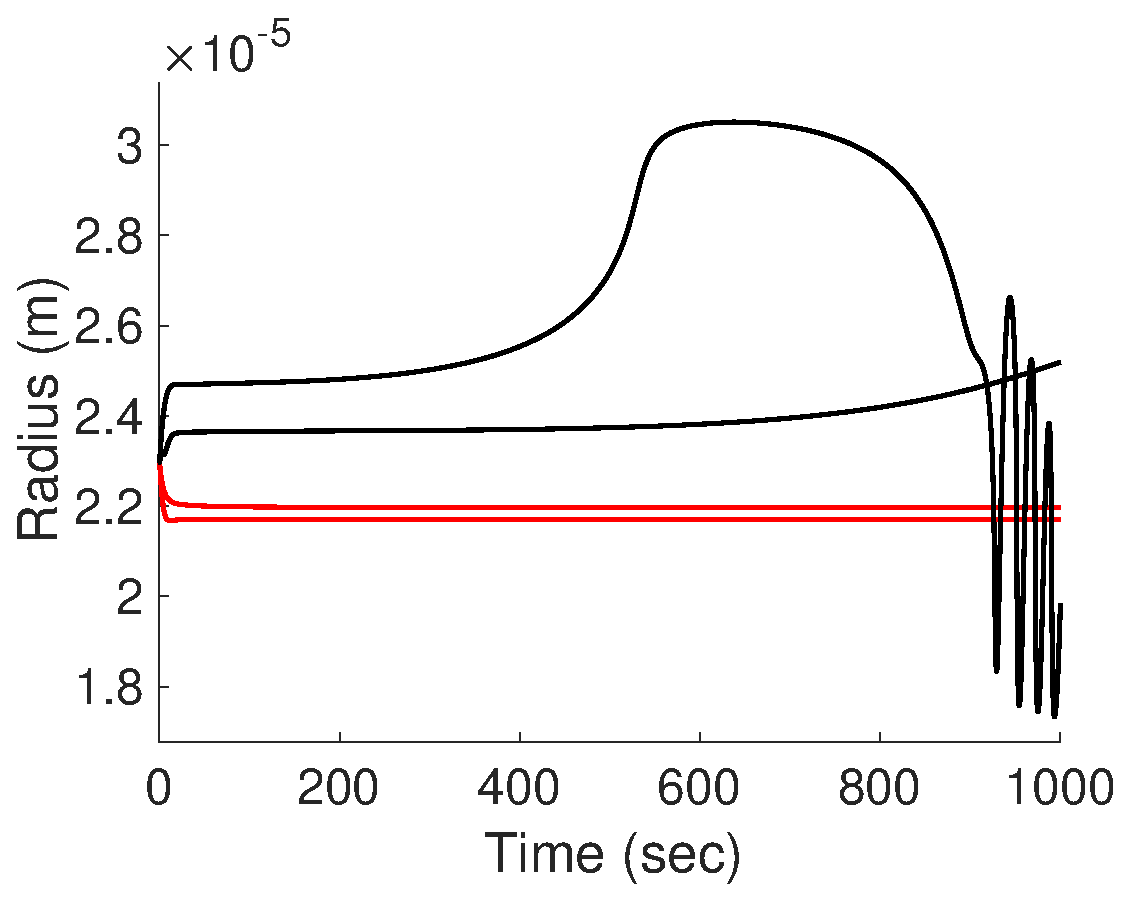
\includegraphics[width=.4 \textwidth]{Figures/Steady_State_Curves.eps}
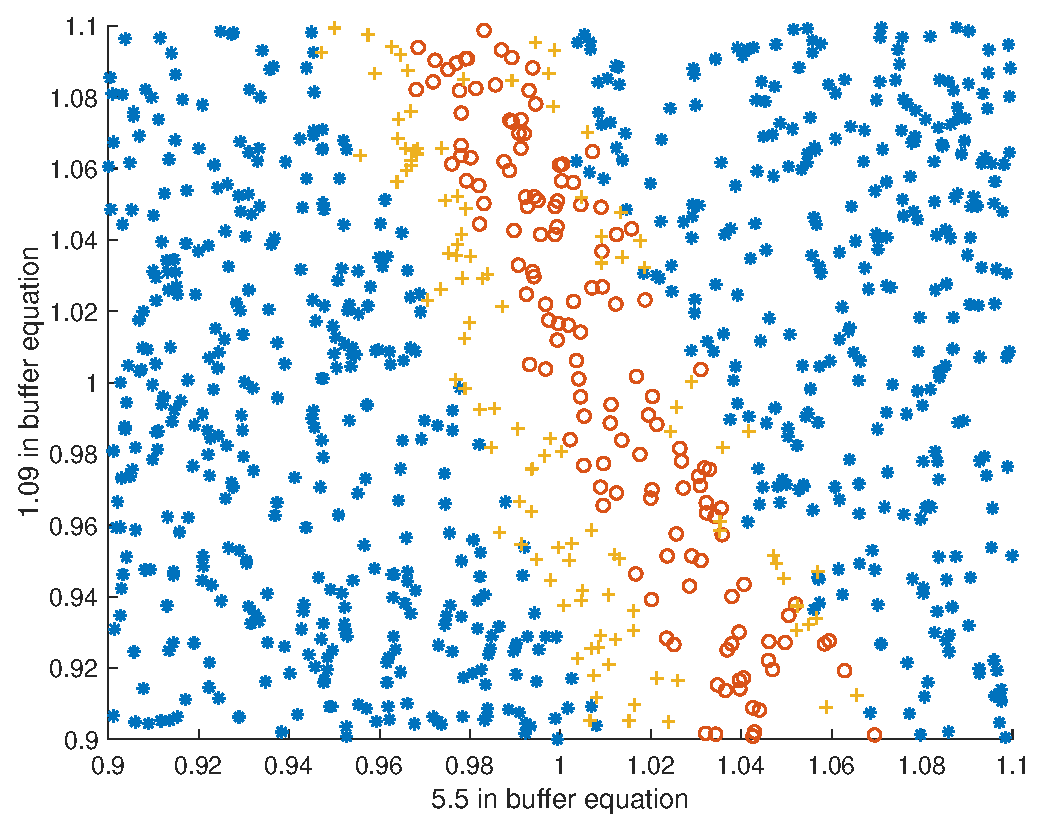
\includegraphics[width=.4 \textwidth]{Figures/First_Iteration_Samples.eps}
\caption{Left: examples of stable (red) and unstable (black) steady state solutions. Right: samples of the buffer parameters using uniform independent sampling. A blue \textcolor{blue}{*} indicates the sample yielded a premature termination of the solver, a yellow \textcolor{yellow}{$\Diamond$} indicates the sample yielded an unstable steady state, a red \textcolor{red}{$\circ$} indicates the sample yielded a stable steady state.}
\label{steady_states}
\end{figure}

Observing this correlation, we use the accepted samples to fit the two buffer parameters with a bivariate Frank copula with beta marginals. The experiment is repeated by sampling the two correlated parameters from this bivariate distribution and all other parameter from their original uniform distributions. After four iterations refining the joint distribution of $(p_1,p_2)$, we were able to generate 902 out of 960 samples which yielded solutions with stable steady states (51 solutions had unstable steady states and 7 had premature solver terminations). This fitted distribution is used for all subsequent analysis. 

Samples are drawn and the model, with a stimulus applied (in two separate cases, the 10 second rectangular pulse and the 16 second stimulus from experimental data), is run for each sample. This results in solutions exhibiting three different physiological regimes; they are displayed in Figure~\ref{solution_regimes} where the radius is plotted as a function of time. The leftmost panel corresponds to the typical case when the radius increases in response to the stimulus and then decreases when it is removed; the center panel corresponds to an atypical case where the radius has an initial decrease in response to the stimulus; the right panel corresponds to another atypical case where the radius reaches another steady state an does not decrease after the stimulus is removed.

\begin{figure}[h]
\centering
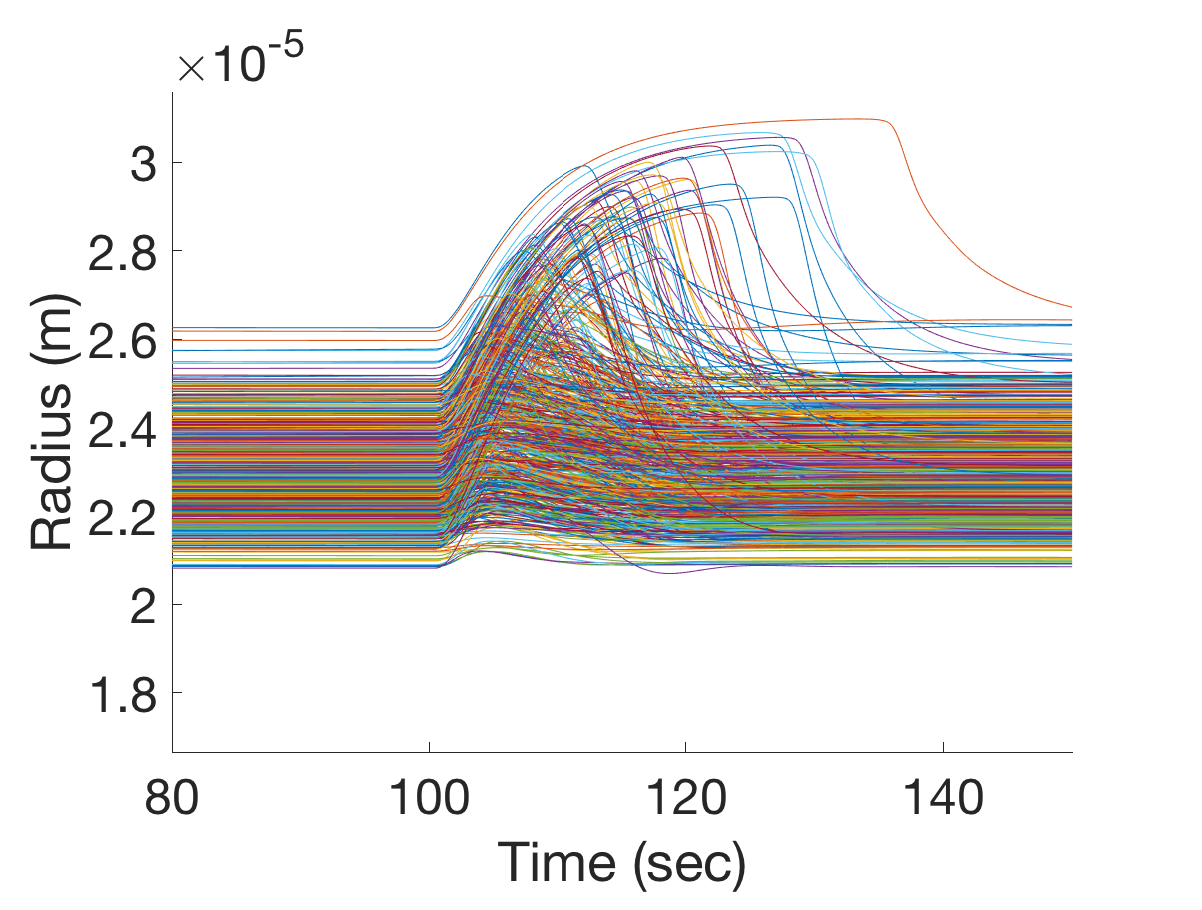
\includegraphics[width=.3 \textwidth]{Figures/Increase_with_Stim_Curves.eps}
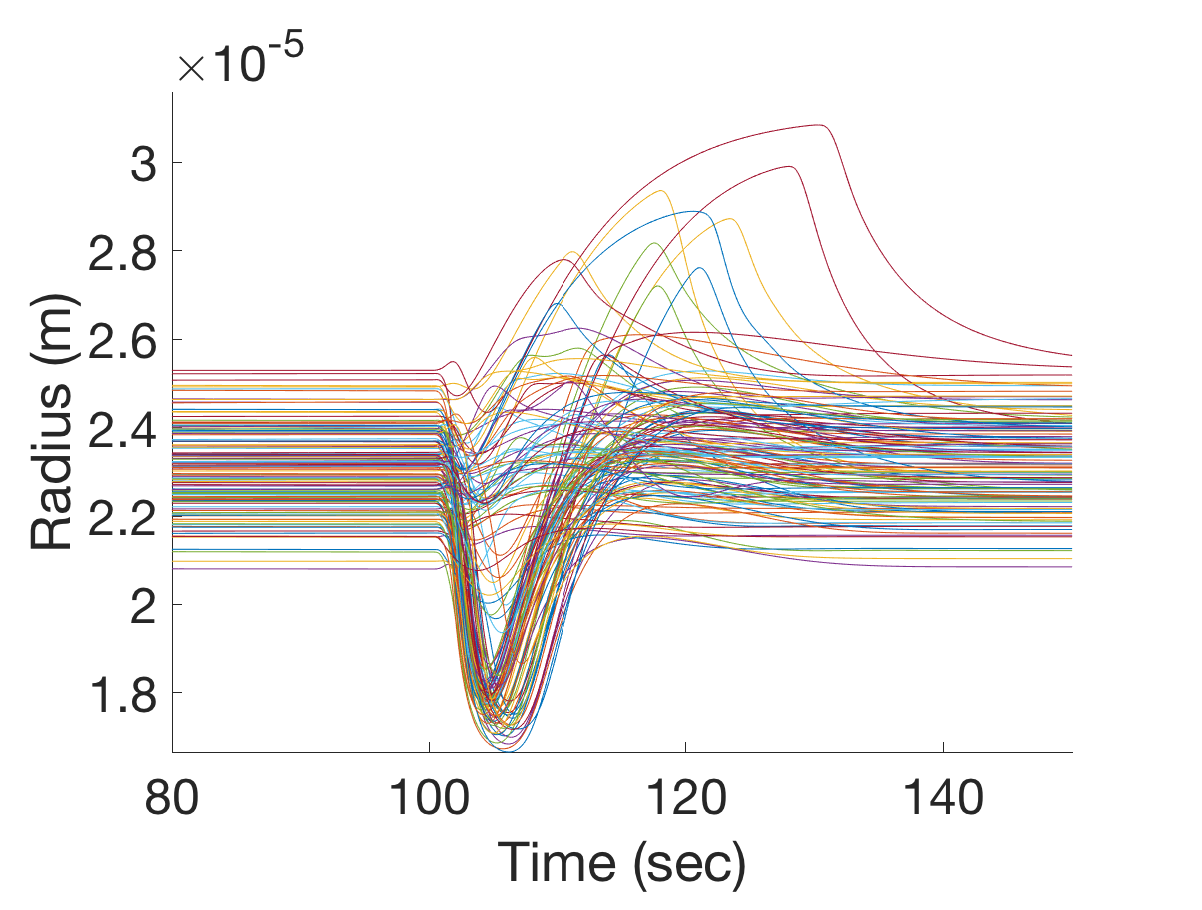
\includegraphics[width=.3 \textwidth]{Figures/Decrease_with_Stim_Curves.eps}
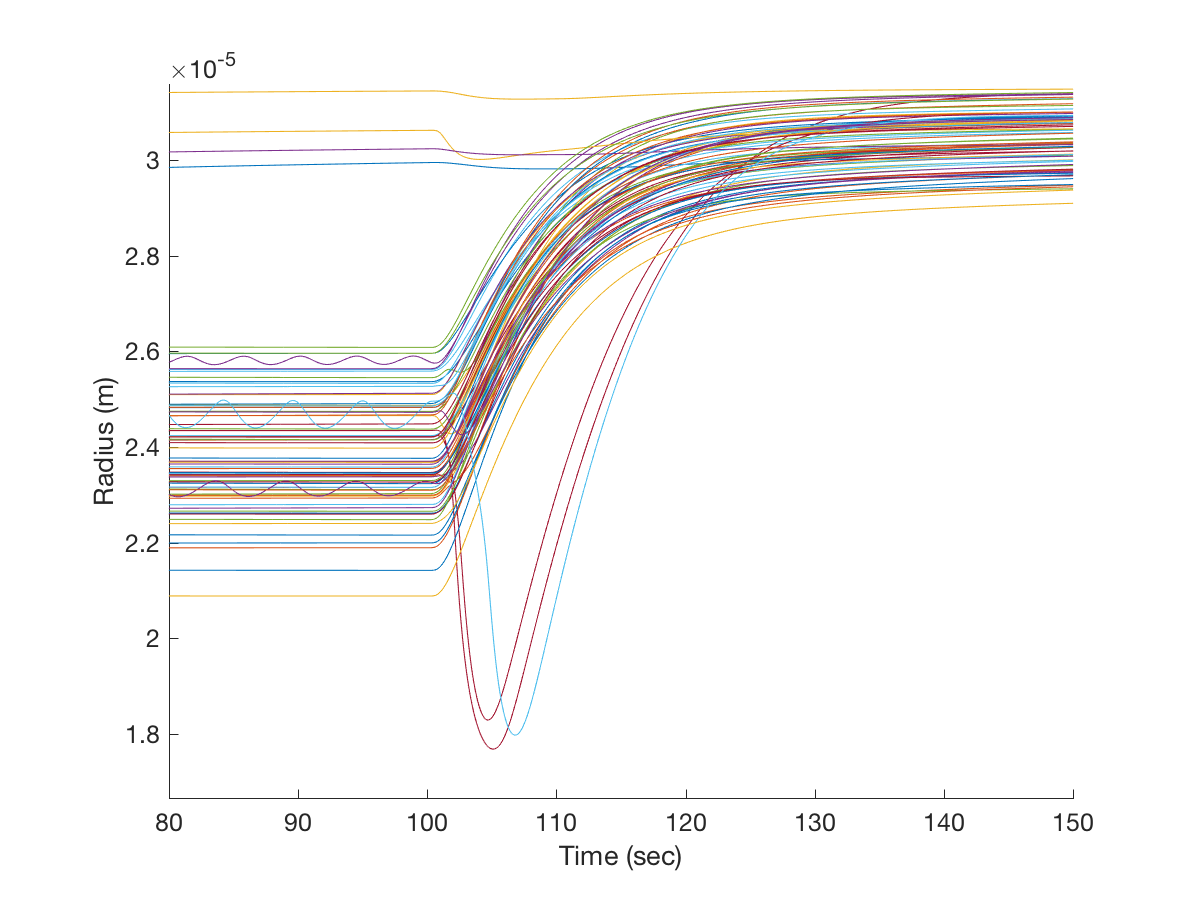
\includegraphics[width=.3 \textwidth]{Figures/Higher_Steady_State.eps}
\caption{Radii corresponding to samples (using the rectangular pulse stimulus). Left: curves an an increase in response to the stimulus; center: curves with a decrease in response to the stimulus; right: curves which settle in a different steady state.}
\label{solution_regimes}
\end{figure}

This article focuses on the typical case so we remove samples where the radius does not increase in response to the stimulus and decrease when it is removed. This processing yields 660 samples for analysis when the rectangular pulse stimulus is applied and 438 samples when the stimulus from experimental data is applied. The results presented below use these samples.

Exploration of the 660 retained samples indicate that atypical cases have higher probability when the parameter which shifts the activation variable for the \pot flux through the soma KDR channel is reduced;
 however, this parameter does not characterize the solution regime by itself; it is likely that the solution regime is characterized by a combination of several parameters. Further sampling and exploration is required to better understand the structure in parameter space which determine the solution regime.



\subsection{ECS $K^+_{mean}$}
\label{sec:qoi_K_ECS_Mean}

Figure~\ref{fig:K_ECS_Mean_rect} and ~\ref{fig:K_ECS_Mean_exp} display results for the average of the ECS potassium as defined in equation (\ref{K_ECS_Mean}) for the rectangular pulse stimulus and experimental pulse stimulus respectively. In the top left panels, predictions of the linear surrogate are plotted against the model values. The sensitivities $L_j$, $j=1,2,\dots,160$, are displayed in the top right panels. Predictions of the PC surrogate are plotted against the model values in the bottom left panels. The total Sobol' indices of the PC surrogate are given in the bottom right panels. 

\begin{figure}[h]
\centering
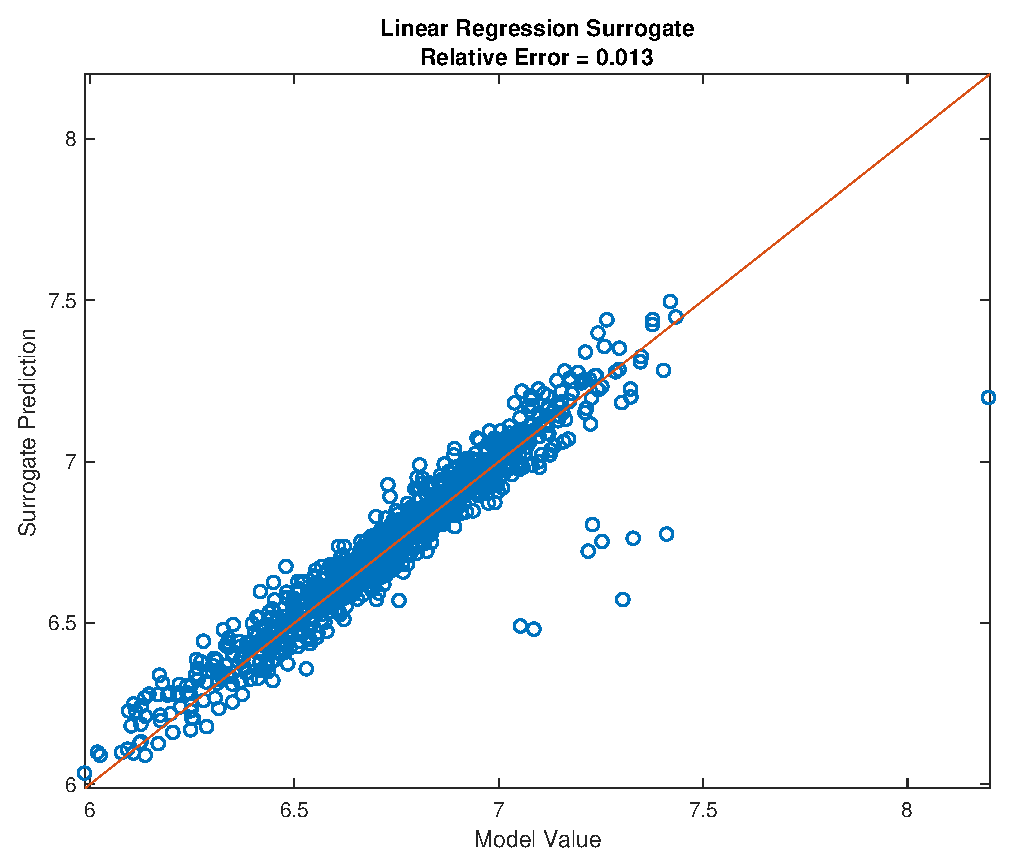
\includegraphics[width=.46 \textwidth]{Figures/K_ECS_Mean_QoI_LR_Prediction_Rectangular.eps}
\hspace{.1 cm}
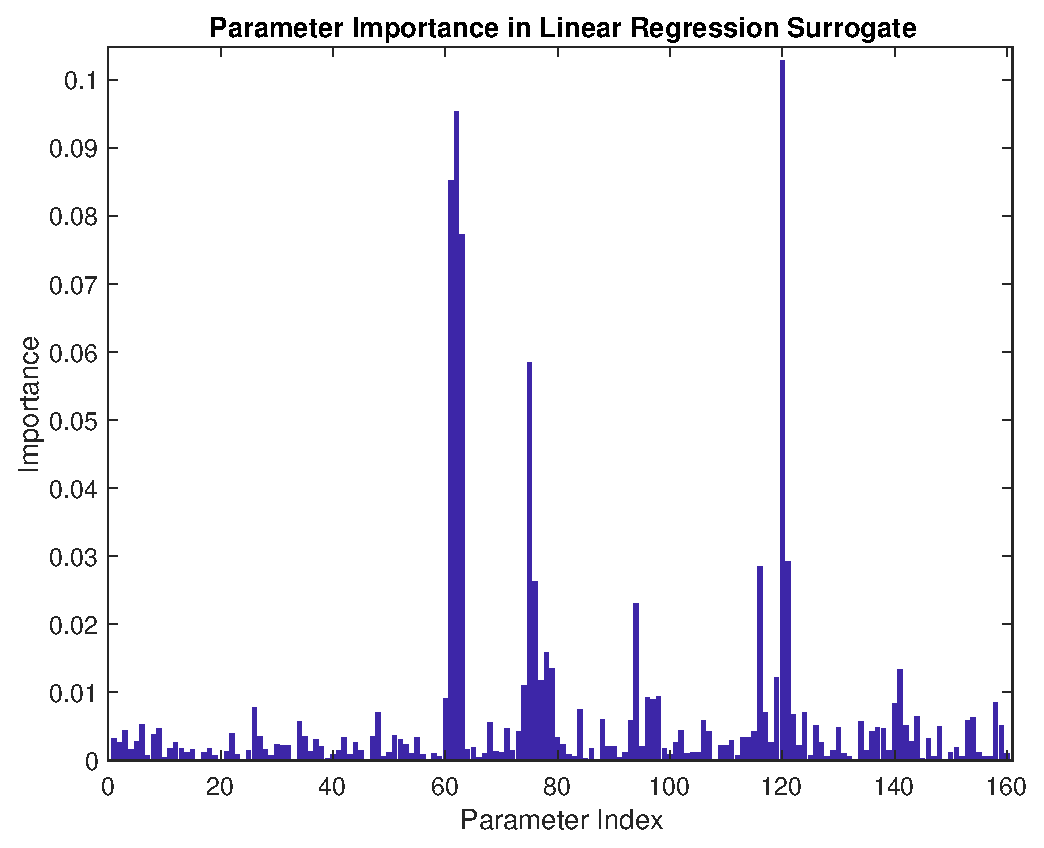
\includegraphics[width=.475 \textwidth]{Figures/K_ECS_Mean_QoI_LR_VI_Rectangular.eps} \\
\vspace{.2 cm}
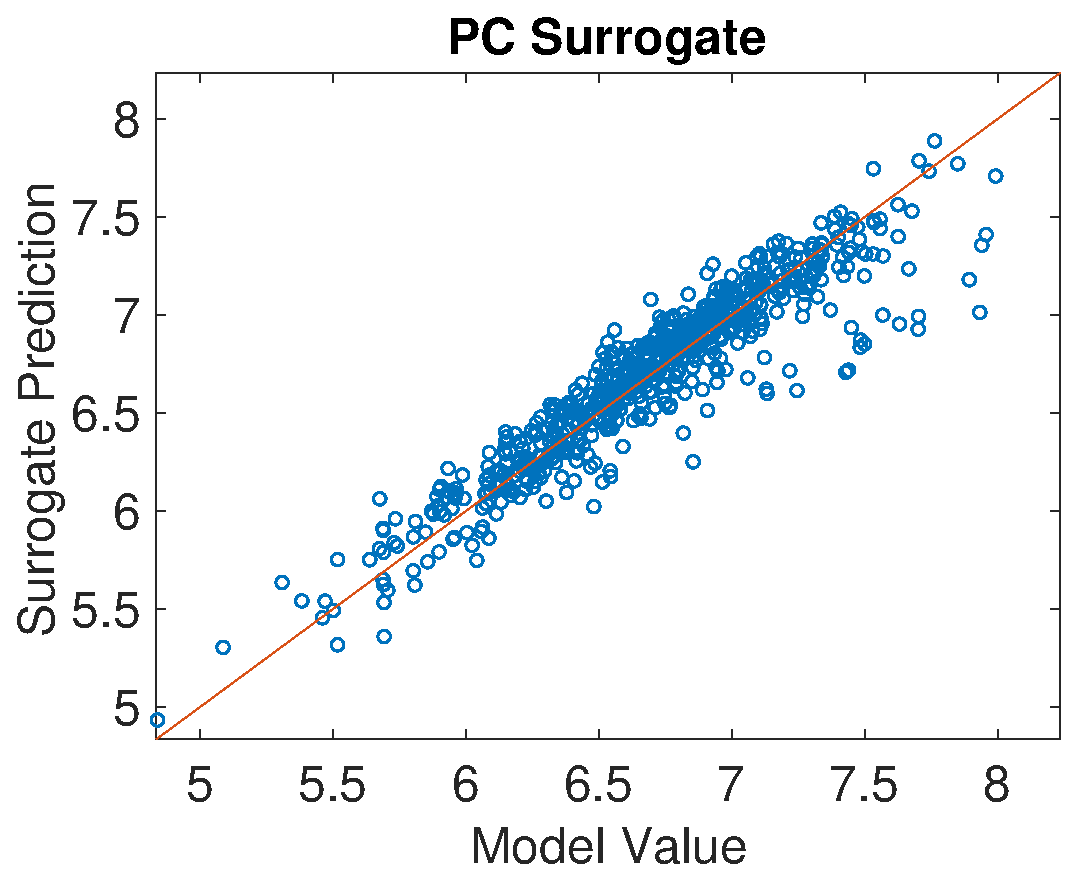
\includegraphics[width=.46 \textwidth]{Figures/K_ECS_Mean_QoI_PCE_Prediction_Rectangular.eps}
\hspace{.1 cm}
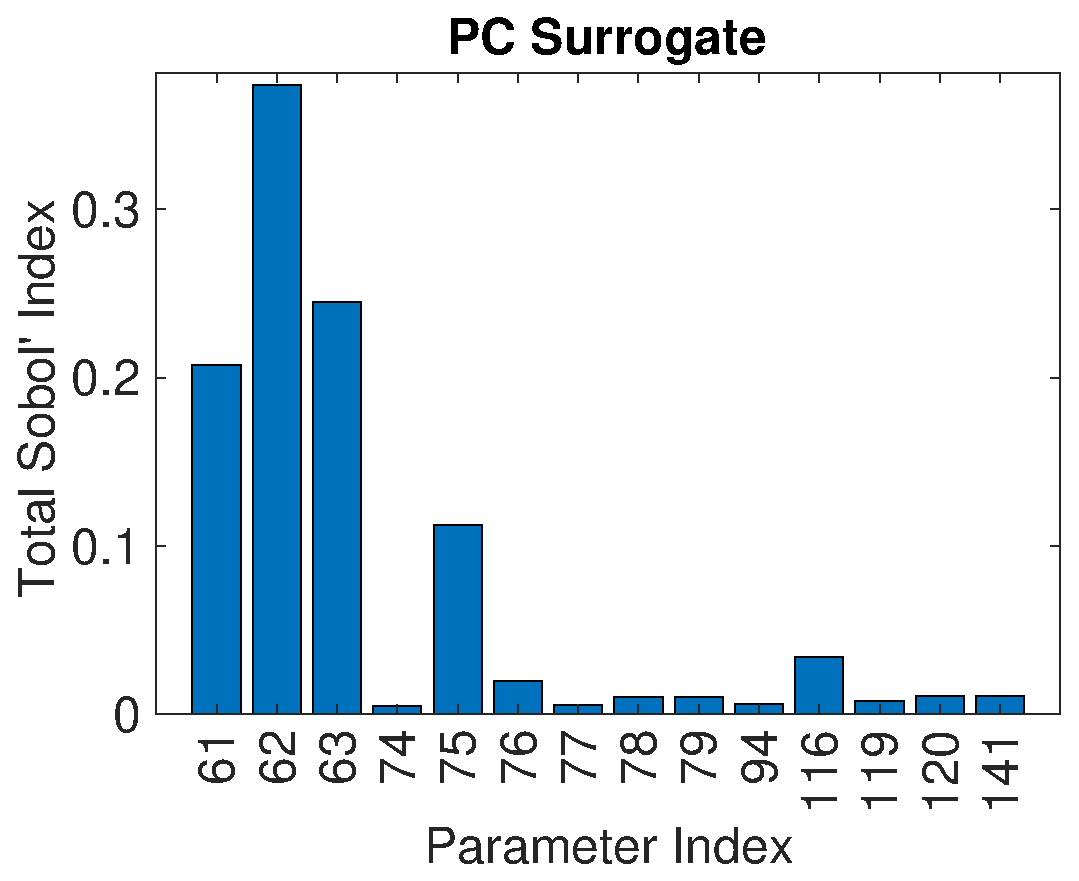
\includegraphics[width=.475 \textwidth]{Figures/K_ECS_Mean_QoI_PCE_SI_Rectangular.eps}
\caption{ECS potassium QoI with a rectangular pulse stimulus. From left to right and top to bottom: linear surrogate predictions, linear surrogate importance measure, PC surrogate predictions, total Sobol' indices for PC surrogate.}
\label{fig:K_ECS_Mean_rect}
\end{figure}
\begin{figure}[h]
\centering
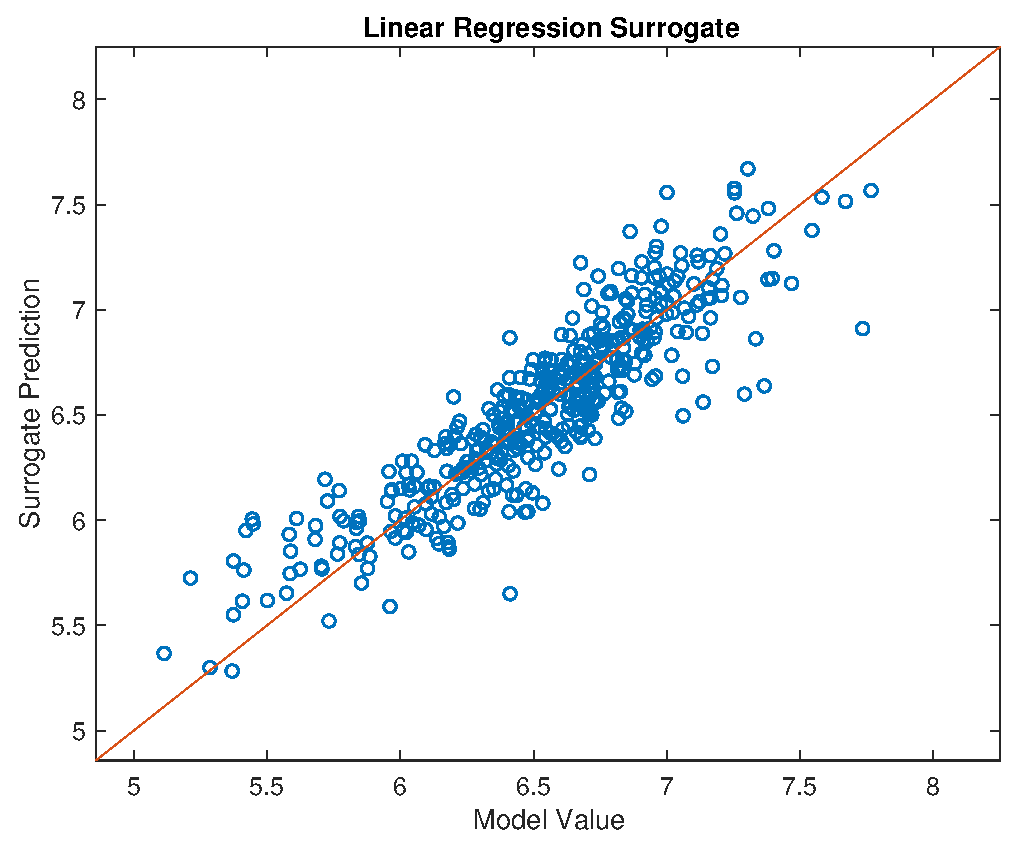
\includegraphics[width=.46 \textwidth]{Figures/K_ECS_Mean_QoI_LR_Prediction_Experimental.eps}
\hspace{.1 cm}
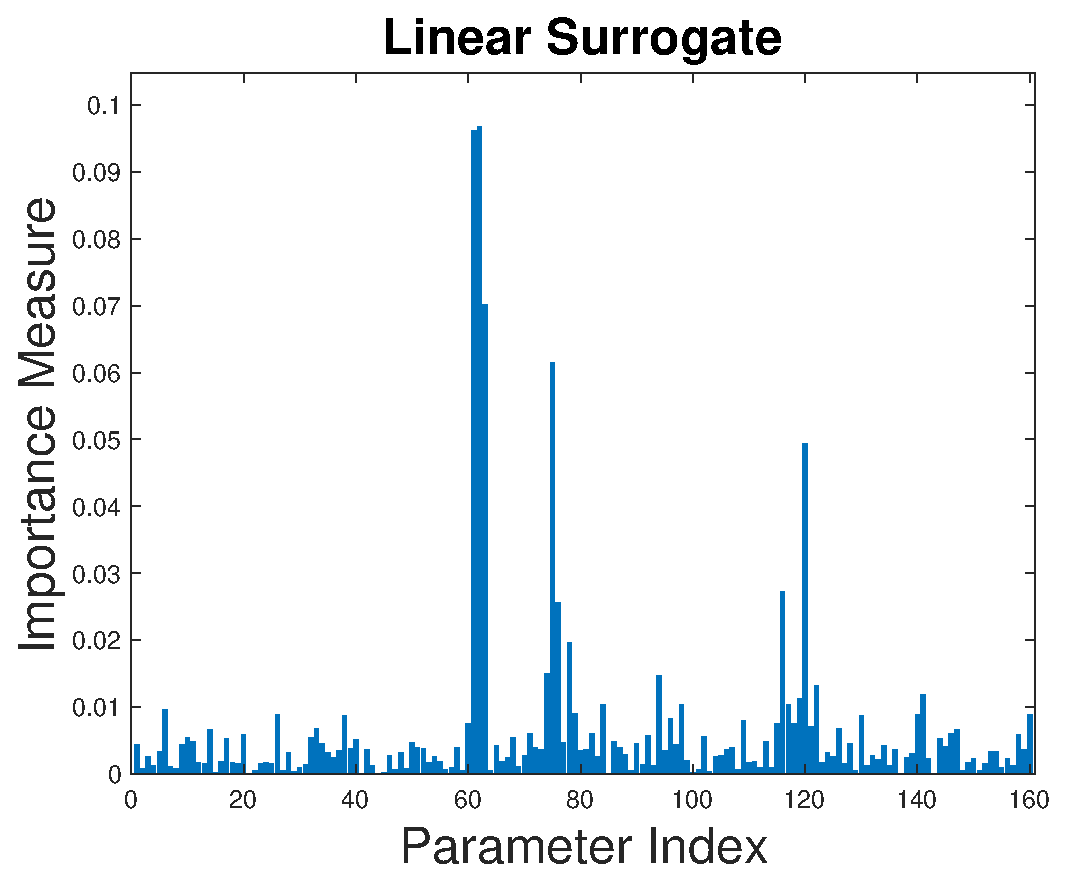
\includegraphics[width=.475 \textwidth]{Figures/K_ECS_Mean_QoI_LR_VI_Experimental.eps} \\
\vspace{.2 cm}
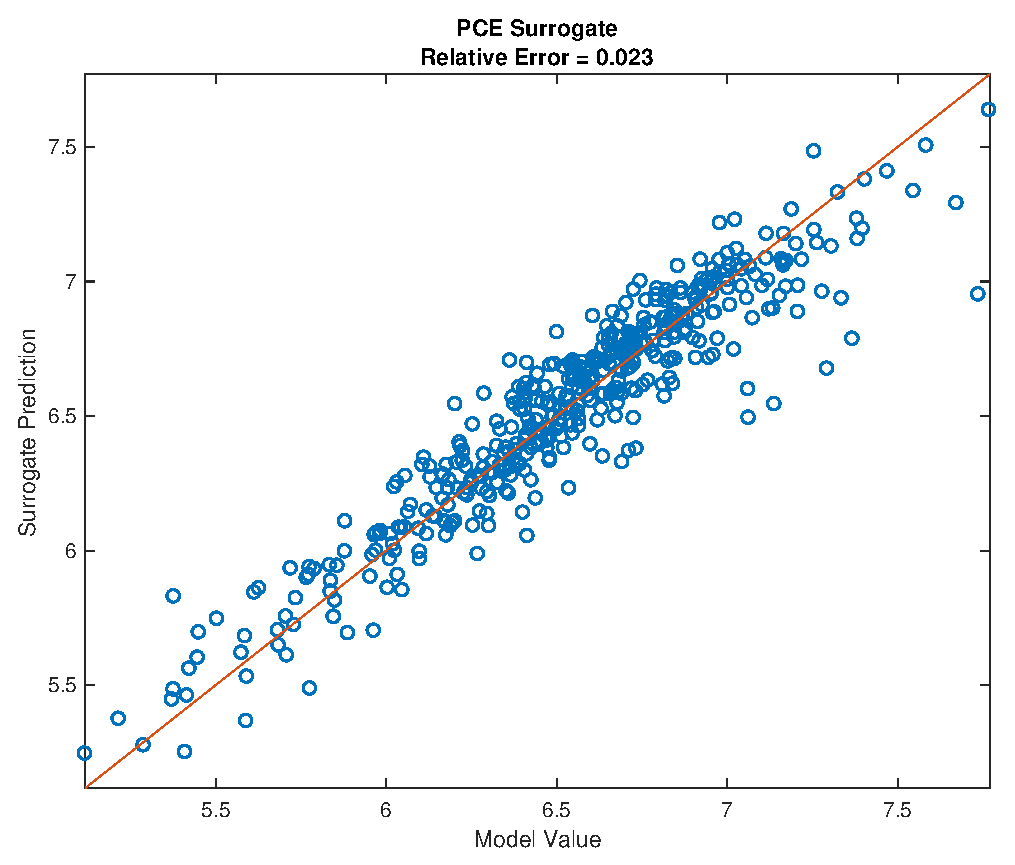
\includegraphics[width=.46 \textwidth]{Figures/K_ECS_Mean_QoI_PCE_Prediction_Experimental.eps}
\hspace{.1 cm}
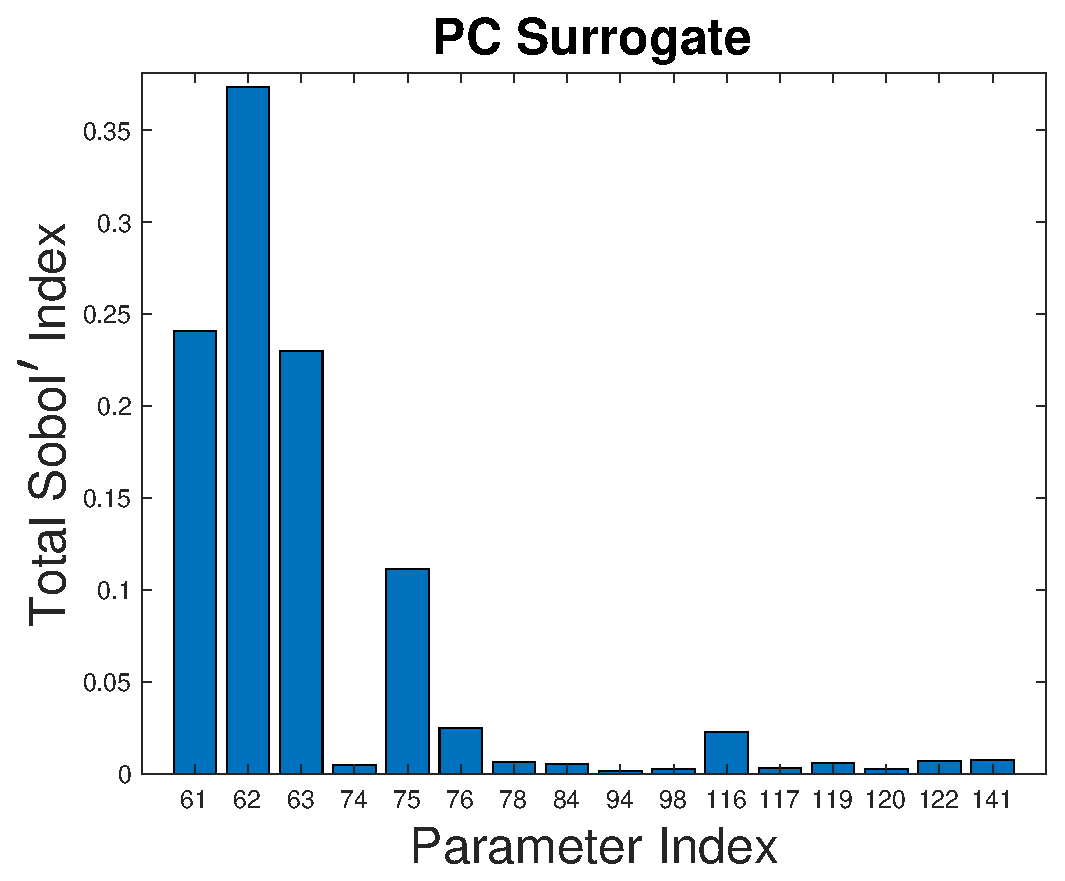
\includegraphics[width=.475 \textwidth]{Figures/K_ECS_Mean_QoI_PCE_SI_Experimental.eps}
\caption{ECS potassium QoI with experimental pulse stimulus. From left to right and top to bottom: linear surrogate predictions, linear surrogate importance measure, PC surrogate predictions, total Sobol' indices for PC surrogate.}
\label{fig:K_ECS_Mean_exp}
\end{figure}

In both cases, Table~\ref{tab:K_ECS_Mean} reports the five most important parameters and their total Sobol' indices. 


%\begin{table}[h]
%\centering
%\ra{1.3}
%\begin{tabular}{cccc}
%\toprule
%Parameter Index & Identification & Total Sobol' Index (rect.) & Total Sobol' Index (exp.)\\
%\midrule
%62 & 0.143 in $m_{4\alpha}$ and $m_{4 \beta}$ &  0.3738 & 0.3732\\
%63 & 5.67 in $m_{4\alpha}$ and $m_{4 \beta}$  &  0.2449 & 0.2297\\
%61 & gKleak\_d in Neuron &0.2074 & 0.2409\\
%75 & 34.9 in $m_{6 \alpha}$ & 0.1124 & 0.1112\\
%116 & dhod in Neuron & 0.0342 & 0.0226\\
% \arrayrulecolor{black}\bottomrule
%\end{tabular}
%\caption{Most influential parameters for the ECS potassium QoI.}
%\label{tab:K_ECS_Mean}
%\end{table}
\begin{table}[h]
\centering
\ra{1.3}
\begin{tabular}{cccc}
\toprule
Parameter Index & Identification & Total Sobol' Index (rect.) & Total Sobol' Index (exp.)\\
\midrule
62 & scaling for activation variable in dendritic NaP channel  &  0.3738 & 0.3732\\
63 &  shift in activation variable in dendritic NaP channel &  0.2449 & 0.2297\\
61 & $K^+$ leak in  Neuron &0.2074 & 0.2409\\
75 & scaling in dendritic KDR channel & 0.1124 & 0.1112\\
116 & half-length of dendrite & 0.0342 & 0.0226\\
 \arrayrulecolor{black}\bottomrule
\end{tabular}
\caption{Most influential parameters for the ECS potassium QoI. The leftmost column is the parameter index displayed in the figures, the left-center column provides a description of the parameter, the right-center column is the total Sobol' index computed for the parameter using the rectangular pulse stimulus, and the right column is the total Sobol' index computed for the parameter using the stimulus from lab experiments.}
\label{tab:K_ECS_Mean}
\end{table}
The top two values in Table \ref{tab:K_ECS_Mean} are scaling and shift parameters for the activation gating variable in the dendrite NaP channel respectively, whose ODE is defined as 
\begin{eqnarray}\label{eqn:m4}
\frac{dm_4}{dt}=m_{4 \alpha}(1-m_4)-m_{4 \beta}m_4, \nonumber \\
m_{4 \alpha}=  \frac{1}{6(1 + exp(-(c_1  v_d + c_2)))},\nonumber \\
m_{4 \beta}= \frac{exp(-(c_1 v_d + c_2))}{6(1 + exp(-(c_1 v_d + c_2)))}.
\end{eqnarray}
The parameters $c_1$ and $c_2$ in \eqref{eqn:m4} correspond to the parameters indexed as 62 and 63 in the results, their nominal values are 0.143 and 5.67, respectively. These effectively define the characteristic time scale and forcing function in the rate equation for the open  probability of the persistent sodium channel. The third most important parameter determines the strength of the  conductance in the \pot leak ion channel. The fourth parameter (parameter index 75), denoted as $c_3$ below, is the shift of the neuron membrane potential in the ODE for the activation variable for the  K flux through dendritic KDR channel, defined as 
\begin{eqnarray}\label{eqn:m6}
m_{6  \alpha}     = 0.016 \left(\frac{v_d + c_3}{1 - exp(-(0.2 * v_d + 0.2c_3))} \right), 
\end{eqnarray}
where the nominal value of $c_3$ is 34.9. As noted above this parameter provides for atypical cases having higher probability when the parameter value is reduced. The final parameter in Table \ref{tab:K_ECS_Mean} is small but corresponds to the assumed half-length of the dendrite. This is not unexpected as the longer the dendrite the larger the total ion flux. 

The results for this specific QoI are similar for both the rectangular pulse and experimental data stimulus. In both cases, the QoI is approximated with reasonable accuracy by a linear model and with higher accuracy by the PC model. The most important parameters are shared in both cases. Notice that parameter $p_1$, defined in \eqref{eqn:buff}, appears to be important in the linear model but unimportant in the PC model. This is because it is strongly correlated with parameter $p_2$ (also defined in defined in \eqref{eqn:buff}), see Figure~\ref{steady_states}, and as a result the coefficient in linear surrogate may be very large because its effect is offset by the effect of $p_2$. To decorrelate inputs, the PC surrogate is build with only $p_1$ instead of both $p_1$ and $p_2$. It subsequently has minimal importance.

The remaining two QoIs also present very similar results for both the rectangular pulse and experimental data stimulus. In the interest of conciseness, we only present figures corresponding to the experimental data stimulus for these two QoIs; Tables~\ref{tab:qoi_vol_flow} and ~\ref{tab:qoi_AM_AMp_Min} give results for both stimuli. 

\subsection{Volumetric Flow Rate}
Figure~\ref{fig:qoi_vol_flow_exp} displays results for the volumetric flow rate in the cerebral tissue defined by (\ref{vol_flow})  in the same manner as Figures~\ref{fig:K_ECS_Mean_rect} and \ref{fig:K_ECS_Mean_exp}. The results correspond to the experimental data stimulus.  Table~\ref{tab:qoi_vol_flow} reports the five most important parameters and their total Sobol' indices. Unsurprisingly, the parameter list contains values found in the SMC/EC compartment of the full model. However, the topmost parameter, $z_4$, is associated with the conductance of the inwardly rectifying SMC KIR channel, $g_{KIR}$, defined as a function of both membrane potential $v_{SMC}$ and the \pot concentration in the perivascular space $[K^+]_{PVS}$, given by 
\begin{eqnarray}
g_{KIR}=exp\left( z_5 v_{SMC}+z_3[K^+]_{PVS}-z_4\right)  \label{eqn:gkir}
\end{eqnarray}
as shown in \cite{Dormanns2015} fitting to the data of \cite{Filosa2006}. $z_4$ shifts the conductance to the right for constant $[K^+]_{PVS}$  concentration in the perivascular space whilst $n_{cross}$ (found in the wallmechanics section of the model) determines the strength of influence of cytosolic $[Ca^{2+}]$ in determining the reaction rate of phosphorylation of myosin \cite{Hai1988}. Although not especially important, $z_2$ shifts the Nernst potential for the KIR channel to the right in the equation
\begin{eqnarray}
v_{KIR}=z_1 [K^+]_{PVS}-z_2. \label{vkir}
\end{eqnarray}

\begin{figure}[h!]
\centering
%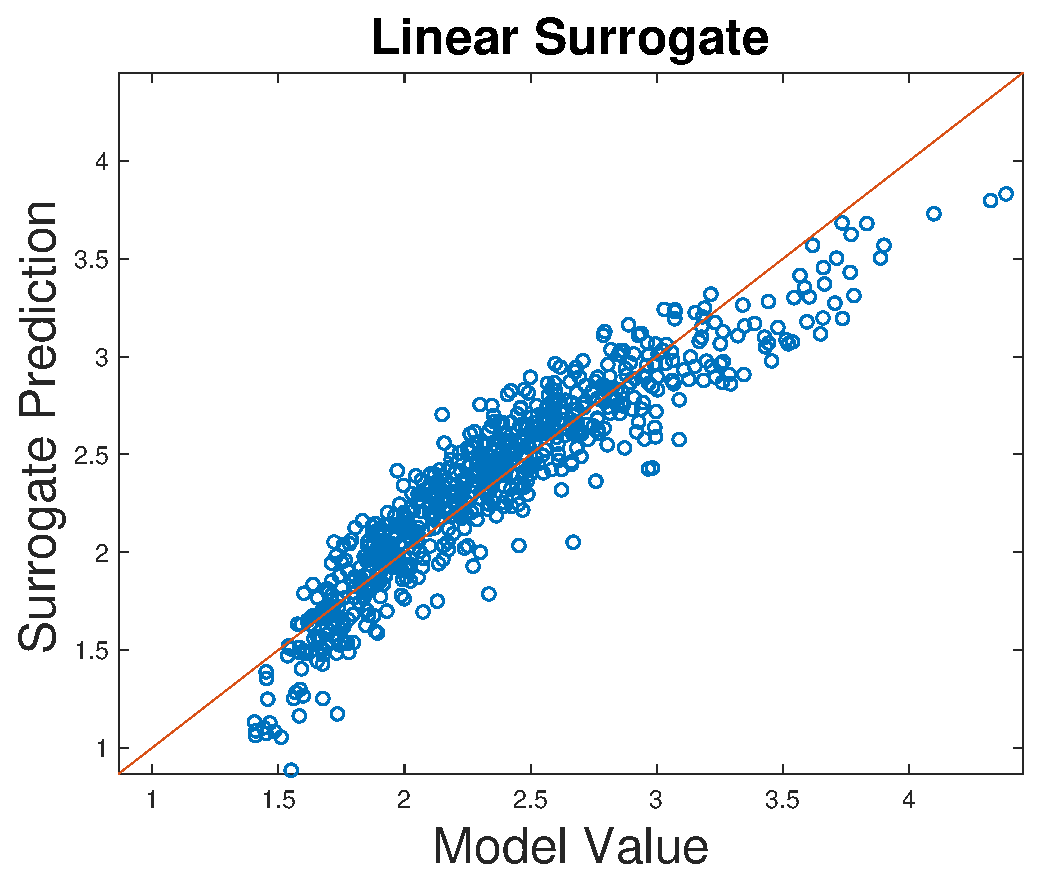
\includegraphics[width=.24 \textwidth]{Figures/Vol_Flow_QoI_LR_Prediction_Rectangular.eps}
%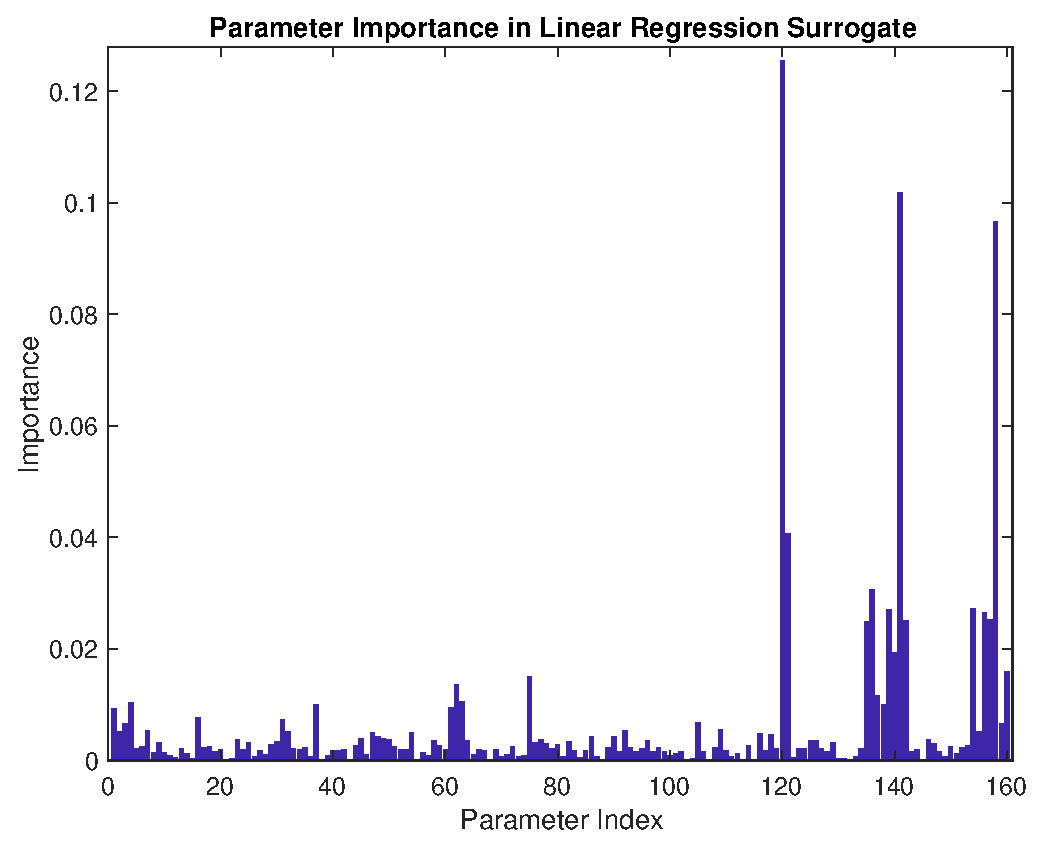
\includegraphics[width=.24 \textwidth]{Figures/Vol_Flow_QoI_LR_VI_Rectangular.eps}
%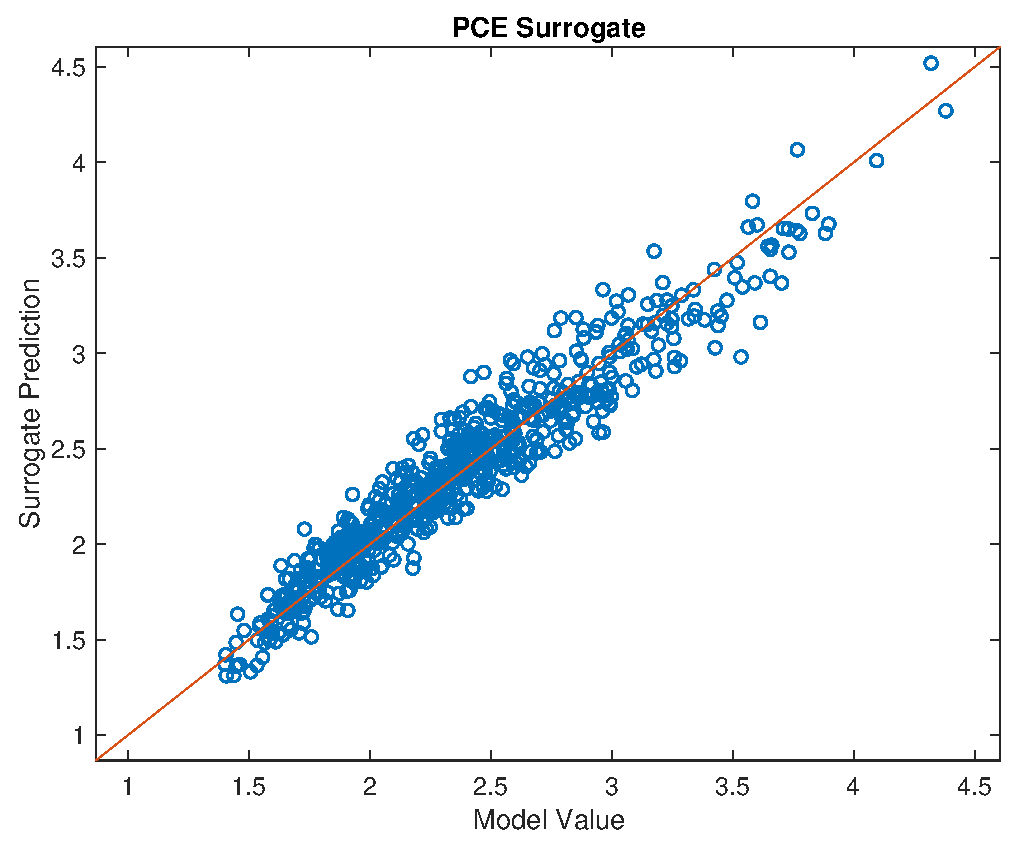
\includegraphics[width=.24 \textwidth]{Figures/Vol_Flow_QoI_PCE_Prediction_Rectangular.eps}
%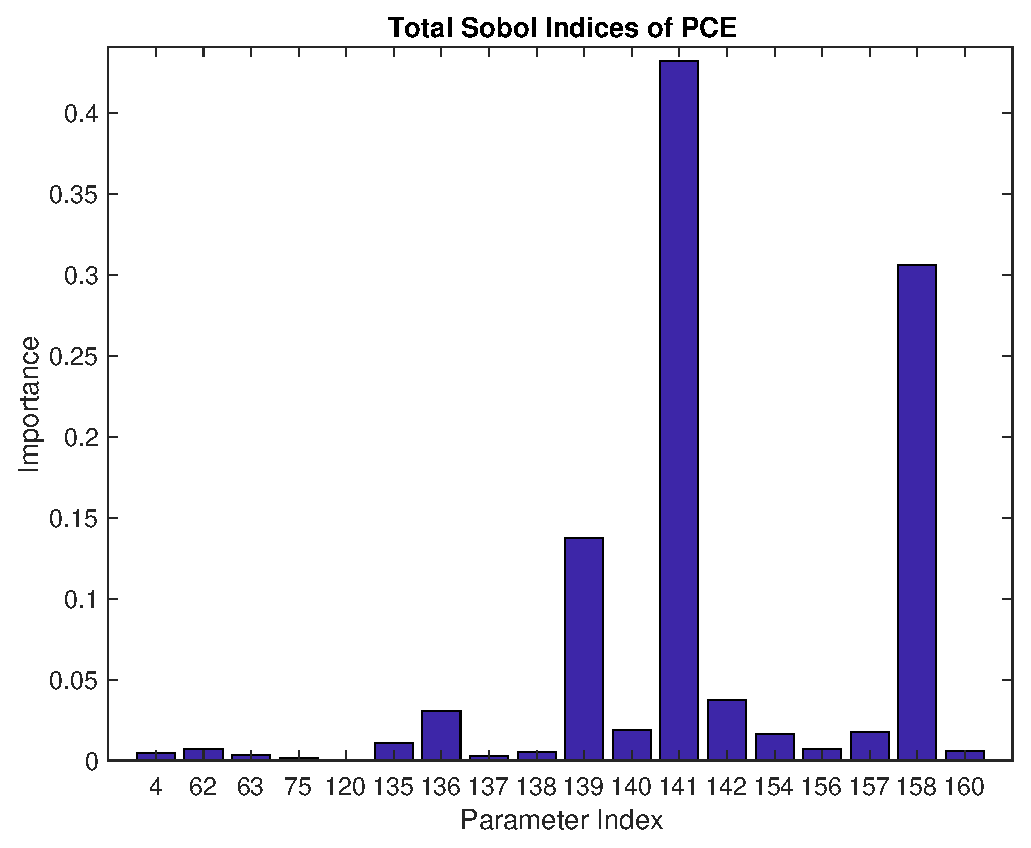
\includegraphics[width=.24 \textwidth]{Figures/Vol_Flow_QoI_PCE_SI_Rectangular.eps}\\
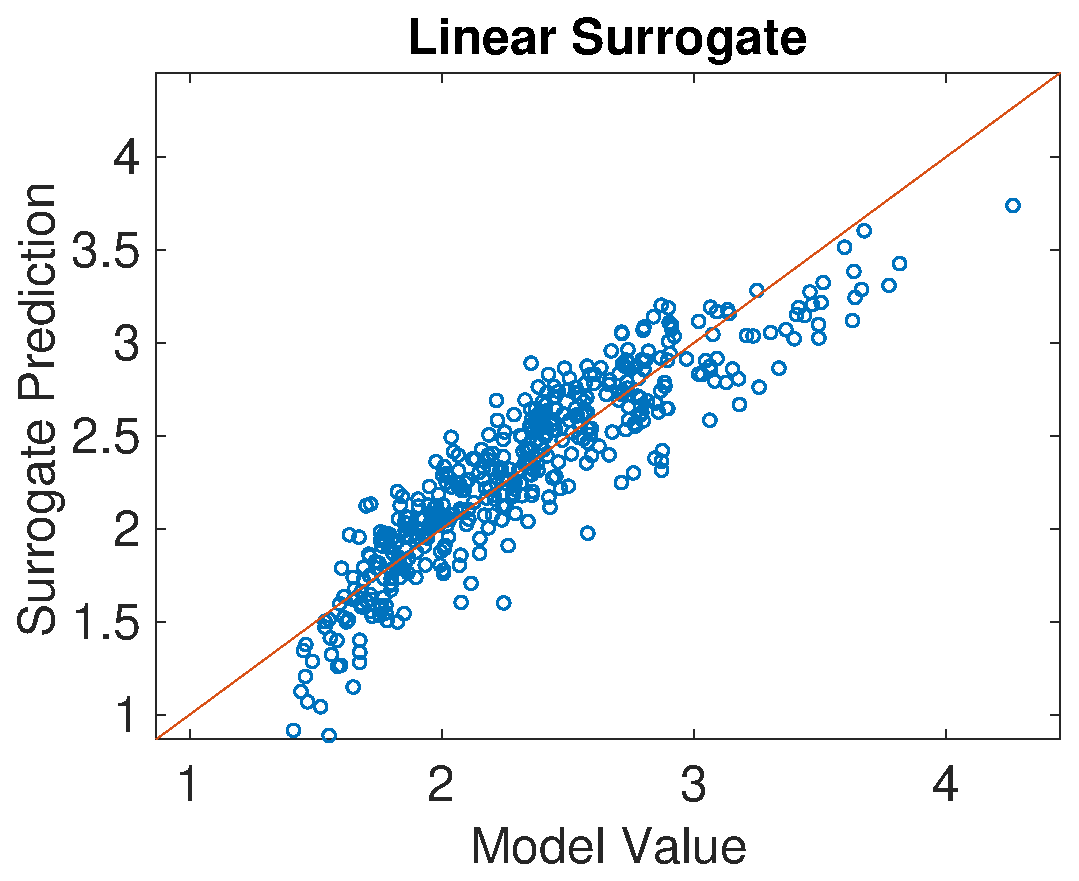
\includegraphics[width=.46 \textwidth]{Figures/Vol_Flow_QoI_LR_Prediction_Experimental.eps}
\hspace{.1 cm}
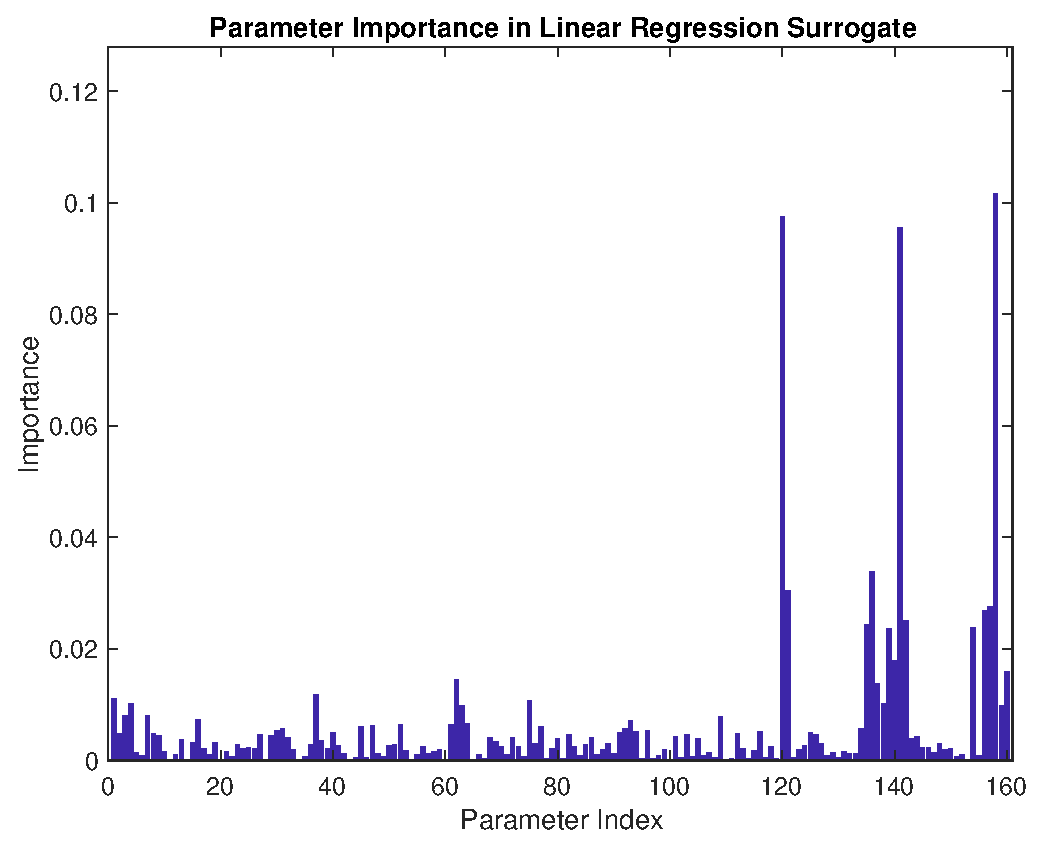
\includegraphics[width=.475 \textwidth]{Figures/Vol_Flow_QoI_LR_VI_Experimental.eps} \\
\vspace{.2 cm}
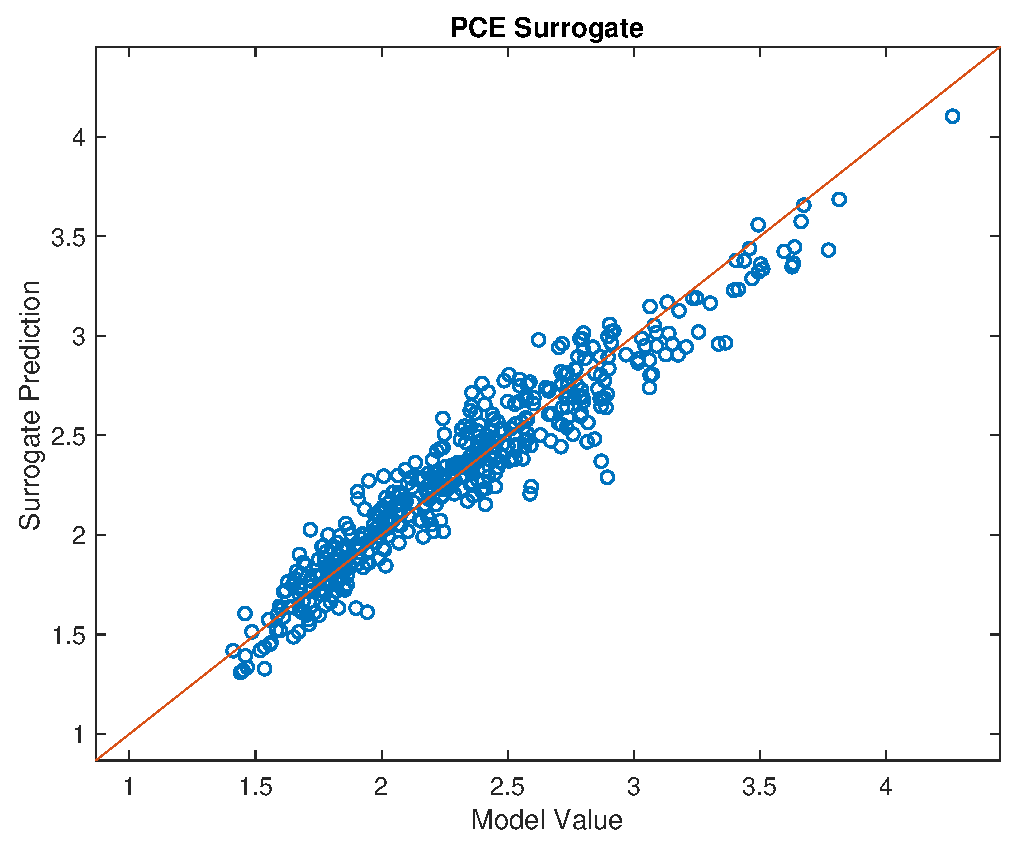
\includegraphics[width=.46 \textwidth]{Figures/Vol_Flow_QoI_PCE_Prediction_Experimental.eps}
\hspace{.1 cm}
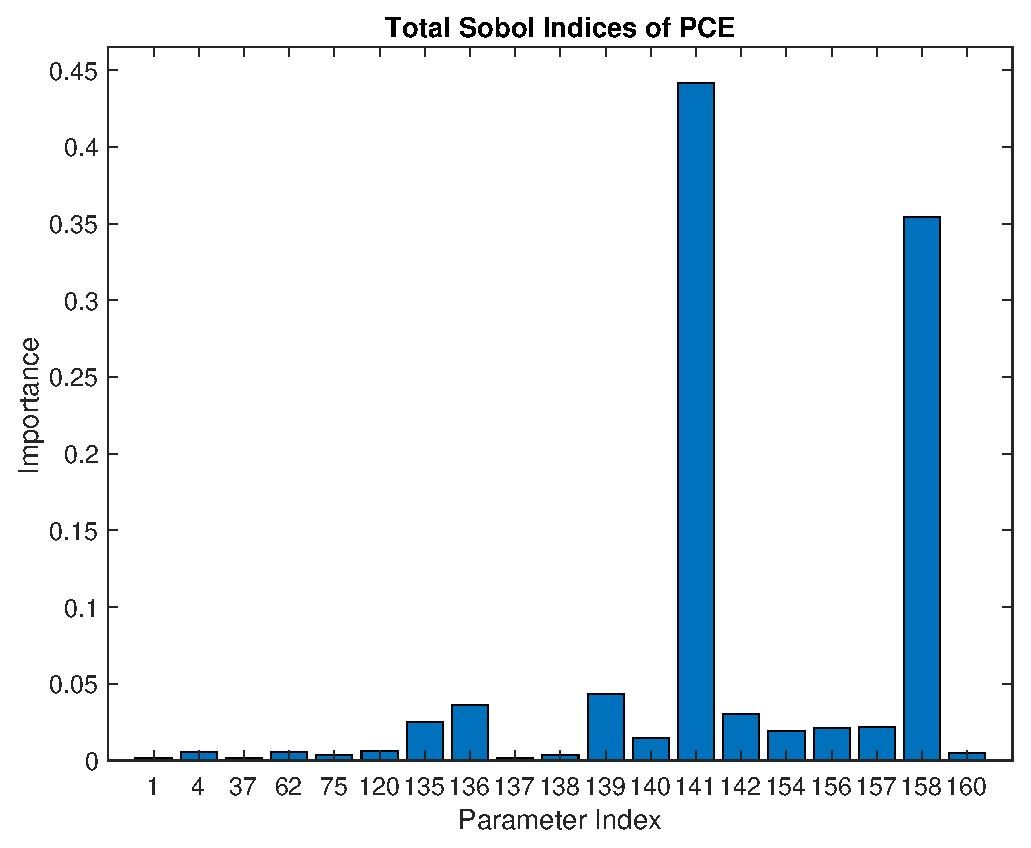
\includegraphics[width=.475 \textwidth]{Figures/Vol_Flow_QoI_PCE_SI_Experimental.eps}
\caption{Volumetric flow rate in the cerebral tissue with experimental pulse stimulus. From left to right and top to bottom: linear surrogate predictions, linear surrogate importance measure, PC surrogate predictions, total Sobol' indices for PC surrogate.}
\label{fig:qoi_vol_flow_exp}
\end{figure}

We again observe reasonably accurate fits by a linear surrogate and improved accuracy by a PC surrogate. The surrogate predictions and important parameters for the rectangular pulse and experimental stimulus closely agree. The influential parameters for the volumetric flow rate in the cerebral tissue are different than those found to be influential for the ECS potassium; an unsurprising result. As in Subsection~\ref{sec:qoi_K_ECS_Mean}, parameter $p_1$ appears important in the linear surrogate but unimportant in the PC surrogate.

\begin{table}[h]
\centering
\ra{1.3}
\begin{tabular}{cccc}
\toprule
Parameter Index & Identification & Total Sobol' Index (rect.) & Total Sobol' Index (exp.)\\
\midrule
141 &  $z_4$ in SMC/EC & 0.4561 & 0.4420\\
158 & $n_{cross}$ in WallMechanics & 0.3311 & 0.3544\\ 
 139 & $z_2$ in SMC/EC & 0.0529 & 0.0436\\
 142 & $z_5$ in SMC/EC &  0.0351 &0.0305\\
  136 & conductance of the $K^+$ channel in SMC/EC & 0.0305 &0.0362\\
   \arrayrulecolor{black}\bottomrule
\end{tabular}
\caption{Most influential parameters for the volumetric flow rate in the cerebral tissue QoI. The leftmost column is the parameter index displayed in the figures, the left-center column provides a description of the parameter, the right-center column is the total Sobol' index computed for the parameter using the rectangular pulse stimulus, and the right column is the total Sobol' index computed for the parameter using the stimulus from lab experiments.}
\label{tab:qoi_vol_flow}
\end{table}

\subsection{$[AM+AM_p]_{min}$}

Figure~\ref{fig:qoi_AM_AMp_Min_exp} displays results for the minimum of the combined concentration of the actin myosin complex with the experimental data stimulus. Table~\ref{tab:qoi_AM_AMp_Min} reports the five most important parameters (ranked by the total Sobol' indices for the rectangular pulse stimulus) and their total Sobol' indices. By comparing Table~\ref{tab:qoi_AM_AMp_Min} and Table~\ref{tab:qoi_vol_flow}, we see that the $[AM+AM_p]_{min}$ and volumetric flow rate QoIs share their four most important parameters. Although at first analysis this should not be surprising it does suggest that the reaction rates of the actin myosin model for vessel contraction/dilation are relatively insensitive to finding the minimum of the contraction force and that the KIR ion channel is a vital component of the model. 
\begin{figure}[h]
\centering
%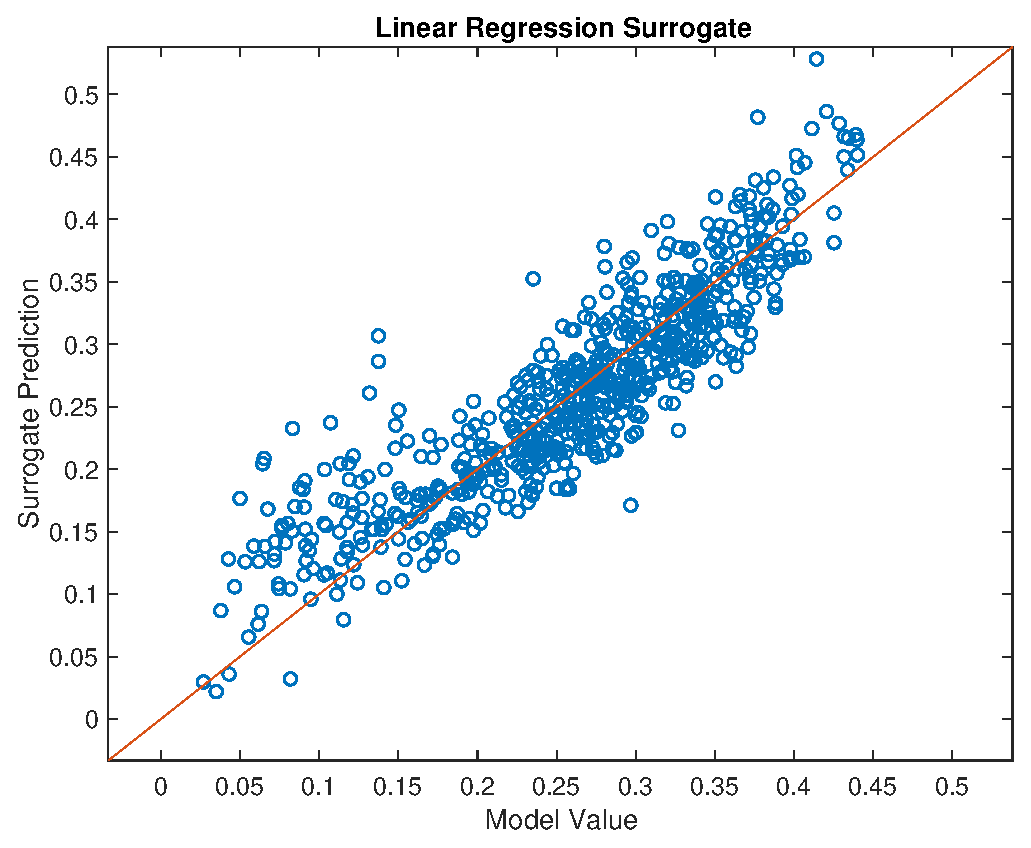
\includegraphics[width=.24 \textwidth]{Figures/AM_AMp_Min_QoI_LR_Prediction_Rectangular.eps}
%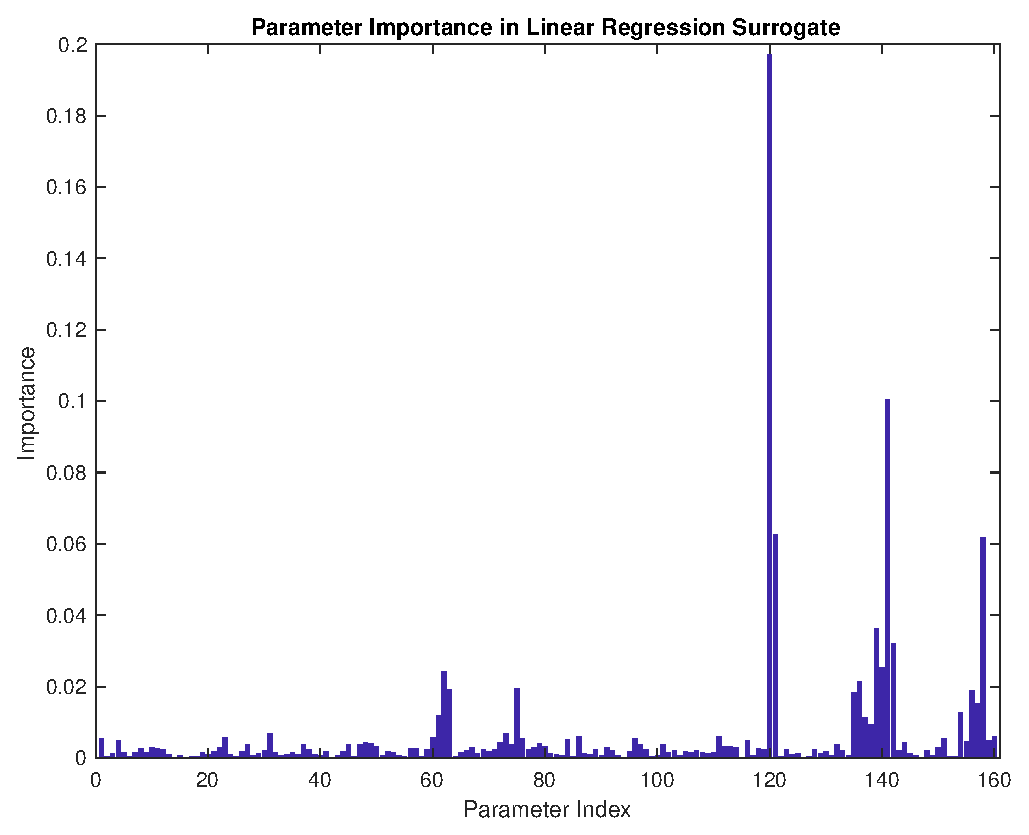
\includegraphics[width=.24 \textwidth]{Figures/AM_AMp_Min_QoI_LR_VI_Rectangular.eps}
%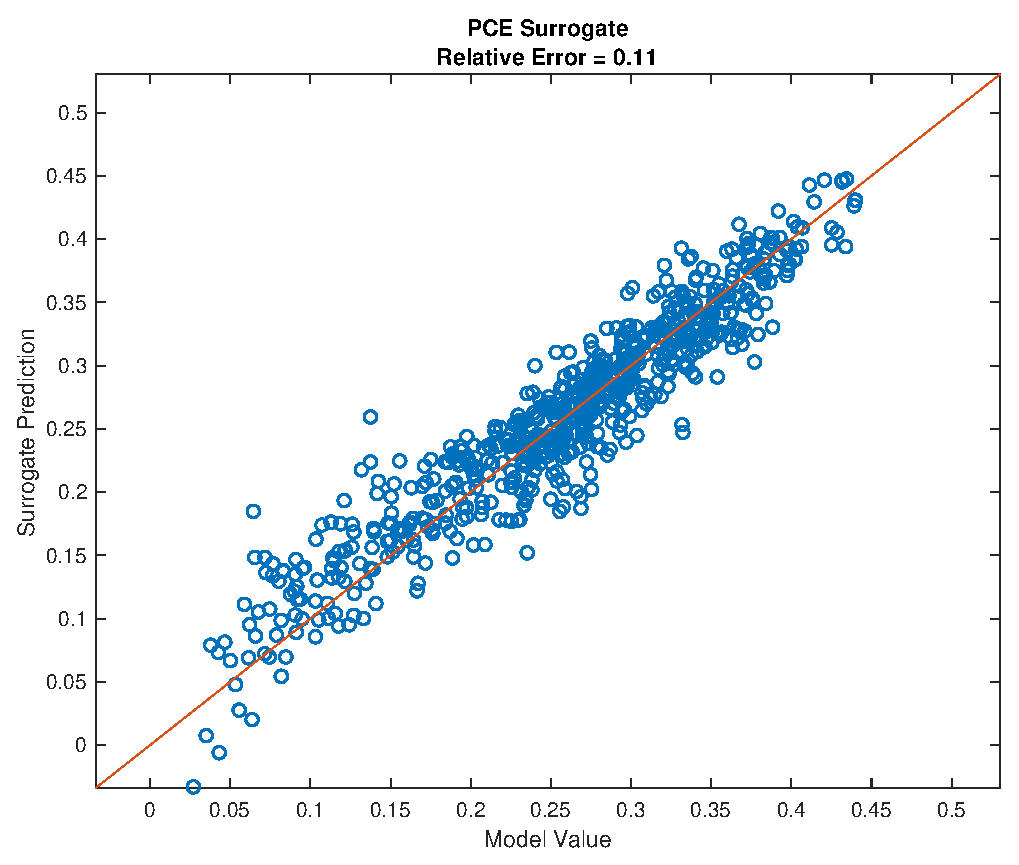
\includegraphics[width=.24 \textwidth]{Figures/AM_AMp_Min_QoI_PCE_Prediction_Rectangular.eps}
%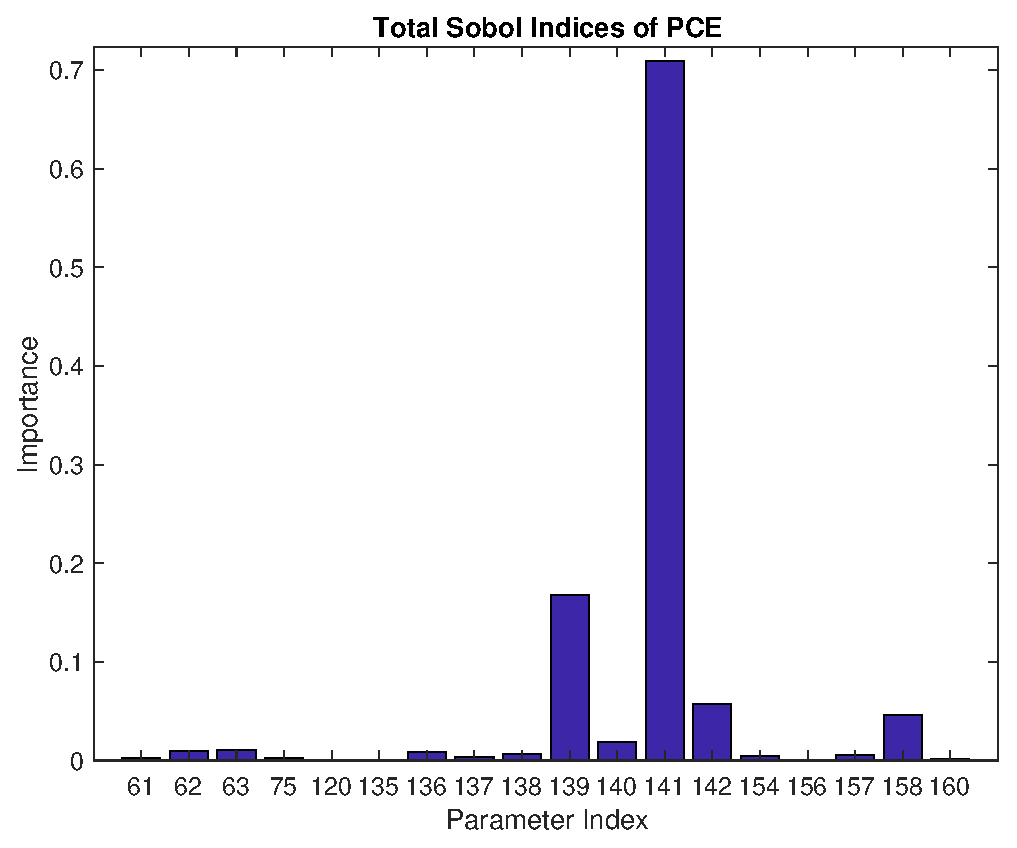
\includegraphics[width=.24 \textwidth]{Figures/AM_AMp_Min_QoI_PCE_SI_Rectangular.eps}\\
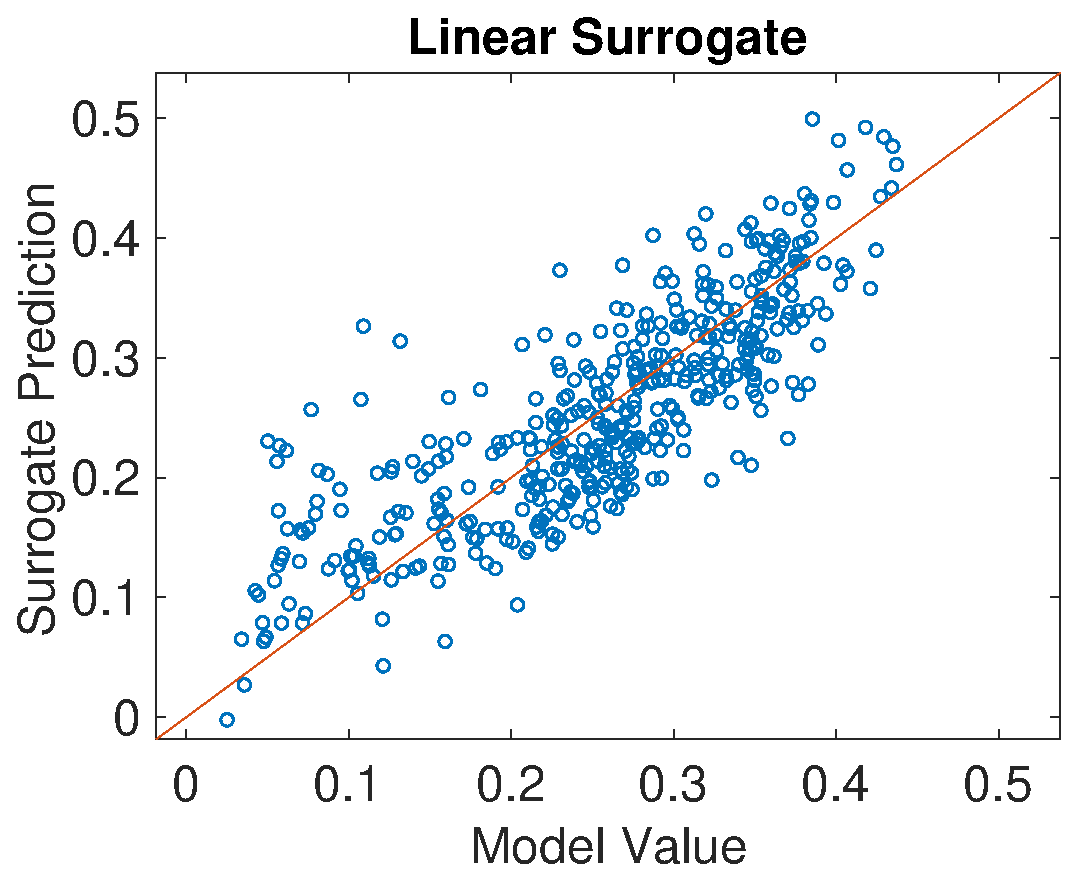
\includegraphics[width=.46 \textwidth]{Figures/AM_AMp_Min_QoI_LR_Prediction_Experimental.eps}
\hspace{.1 cm}
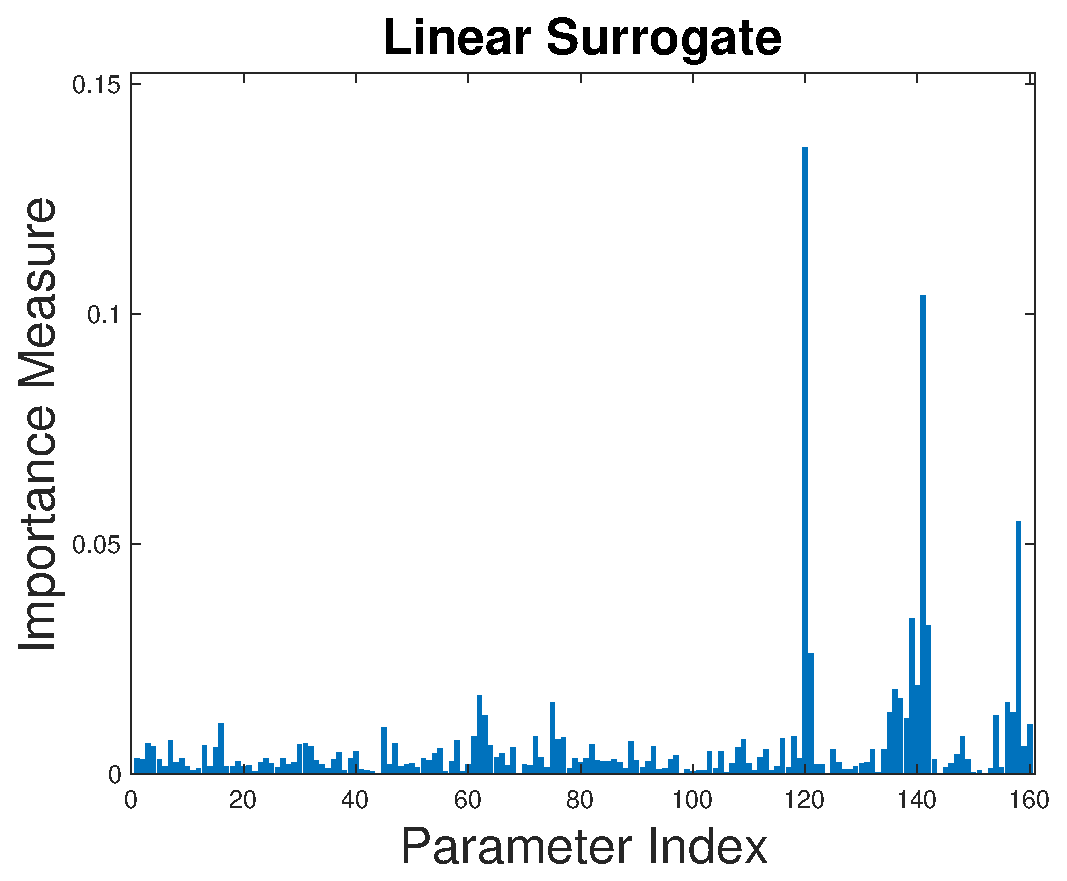
\includegraphics[width=.475 \textwidth]{Figures/AM_AMp_Min_QoI_LR_VI_Experimental.eps} \\
\vspace{.2 cm}
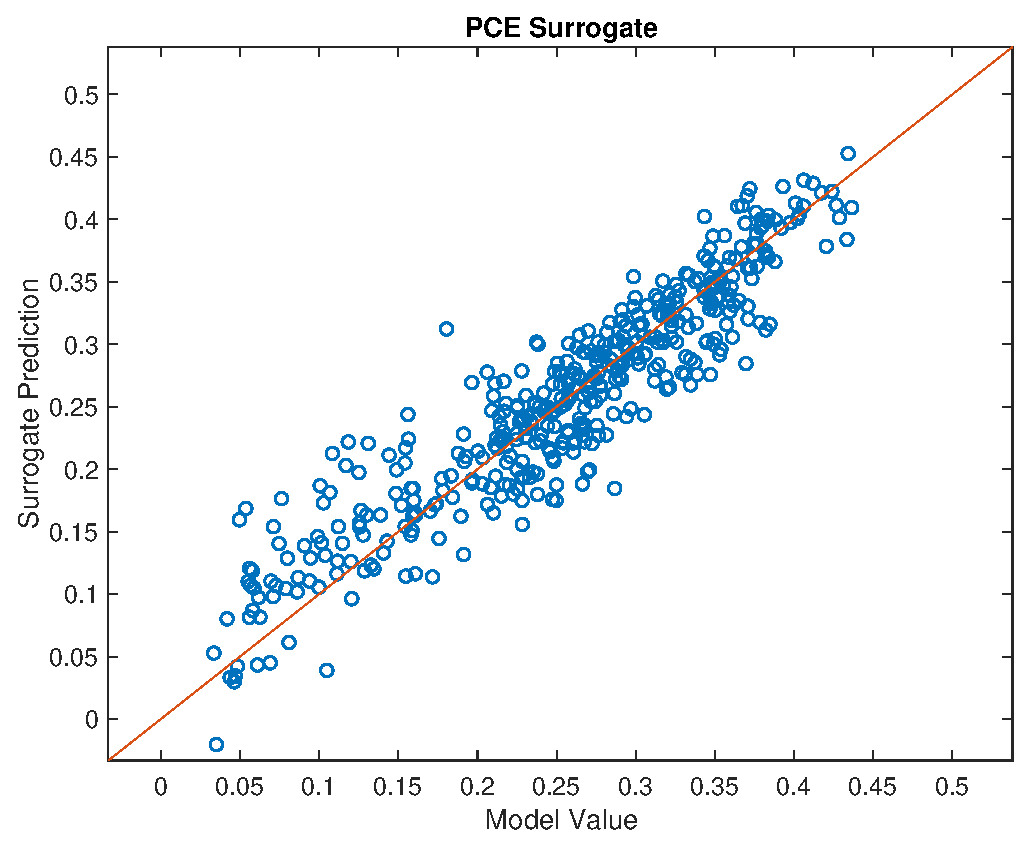
\includegraphics[width=.46 \textwidth]{Figures/AM_AMp_Min_QoI_PCE_Prediction_Experimental.eps}
\hspace{.1 cm}
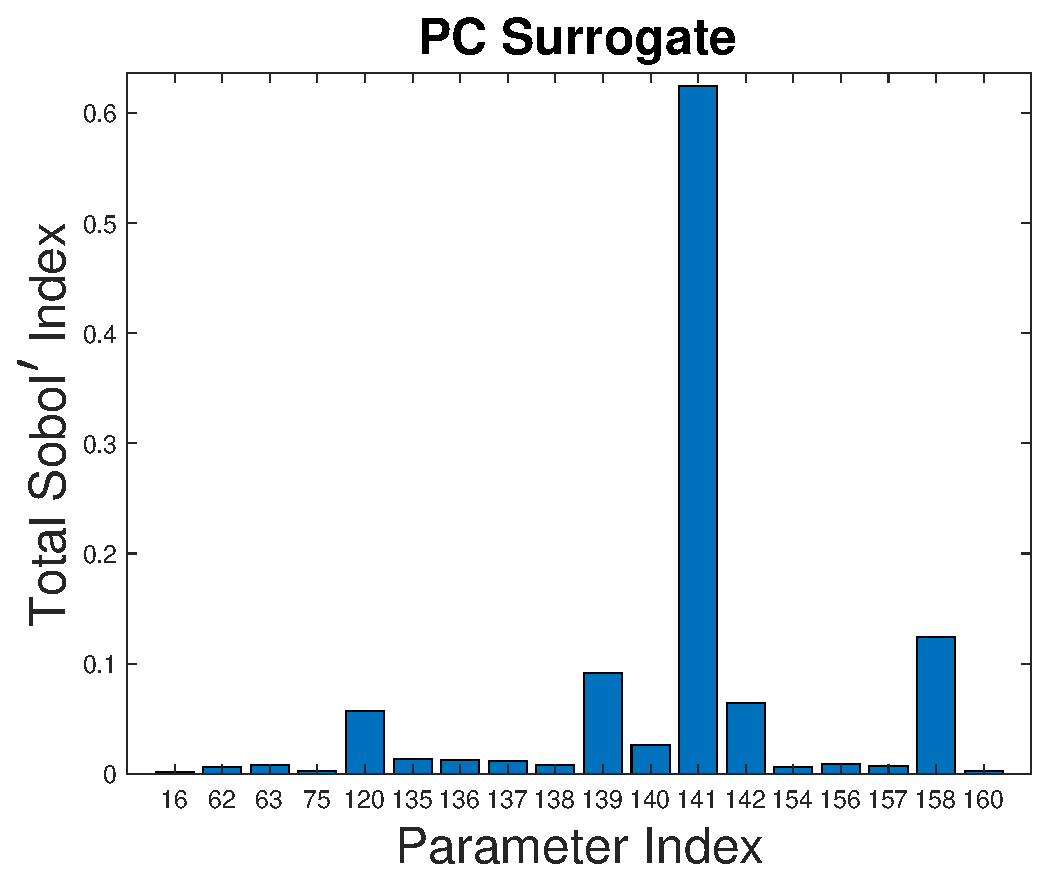
\includegraphics[width=.475 \textwidth]{Figures/AM_AMp_Min_QoI_PCE_SI_Experimental.eps}
\caption{Minimum of the combined concentration of the actin myosin complex with experimental pulse stimulus. From left to right and top to bottom: linear surrogate predictions, linear surrogate importance measure, PC surrogate predictions, total Sobol' indices for PC surrogate.}
\label{fig:qoi_AM_AMp_Min_exp}
\end{figure}

The linear surrogate does not perform as well for this QoI; however, the PC surrogate is far more accurate; this highlights the nonlinearity of this particular QoI. The subset of parameters used in the PC surrogate differs for the rectangular pulse and experimental stimulus cases, but the most important parameters, as measured by the total Sobol' indices, agree. The most influential parameters for the minimum of the combined concentration of the actin myosin complex coincide with those for the volumetric flow rate in the cerebral tissue, an unsurprising result since both QoI are related to the wall mechanics. As in the previous results, parameter $p_1$ appears important in the linear surrogate but unimportant in the PC surrogate.

\begin{table}[h]
\centering
\ra{1.3}
\begin{tabular}{cccc}
\toprule
Parameter Index & Identification & Total Sobol' Index (rect.) & Total Sobol' Index (exp.)\\
\midrule
141 & $z_4$ in SMCEC & 0.6203 & 0.6242\\
158 & $n_{cross}$ in WallMechanics & 0.1488 &0.1239\\
139 &  $z_2$ in SMCEC & 0.0954 &0.0918\\
142 & $z_5$ in SMCEC & 0.0629 & 0.0644\\
140 & $z_3$ in SMCEC & 0.0273 &0.0261\\
 \arrayrulecolor{black}\bottomrule
\end{tabular}
\caption{Most influential parameters for the combined concentration of the actin myosin complex QoI. The leftmost column is the parameter index displayed in the figures, the left-center column provides a description of the parameter, the right-center column is the total Sobol' index computed for the parameter using the rectangular pulse stimulus, and the right column is the total Sobol' index computed for the parameter using the stimulus from lab experiments.}
\label{tab:qoi_AM_AMp_Min}
\end{table}

%\section{Extra figures we probably won't include}
%\subsection{$AM_p$ Time Lag}
%
%\begin{figure}[h]
%\centering
%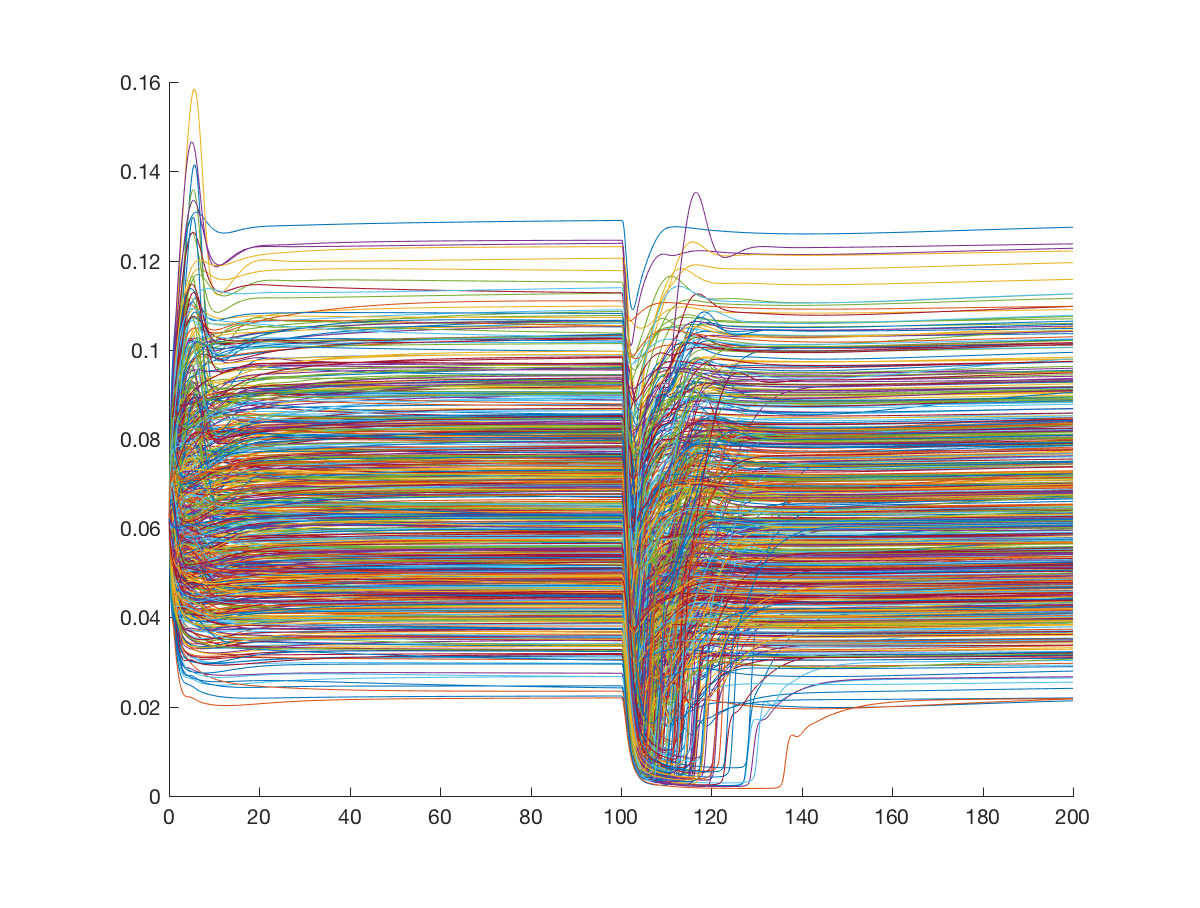
\includegraphics[width=.49 \textwidth]{Figures/AMp_Curves.eps}
%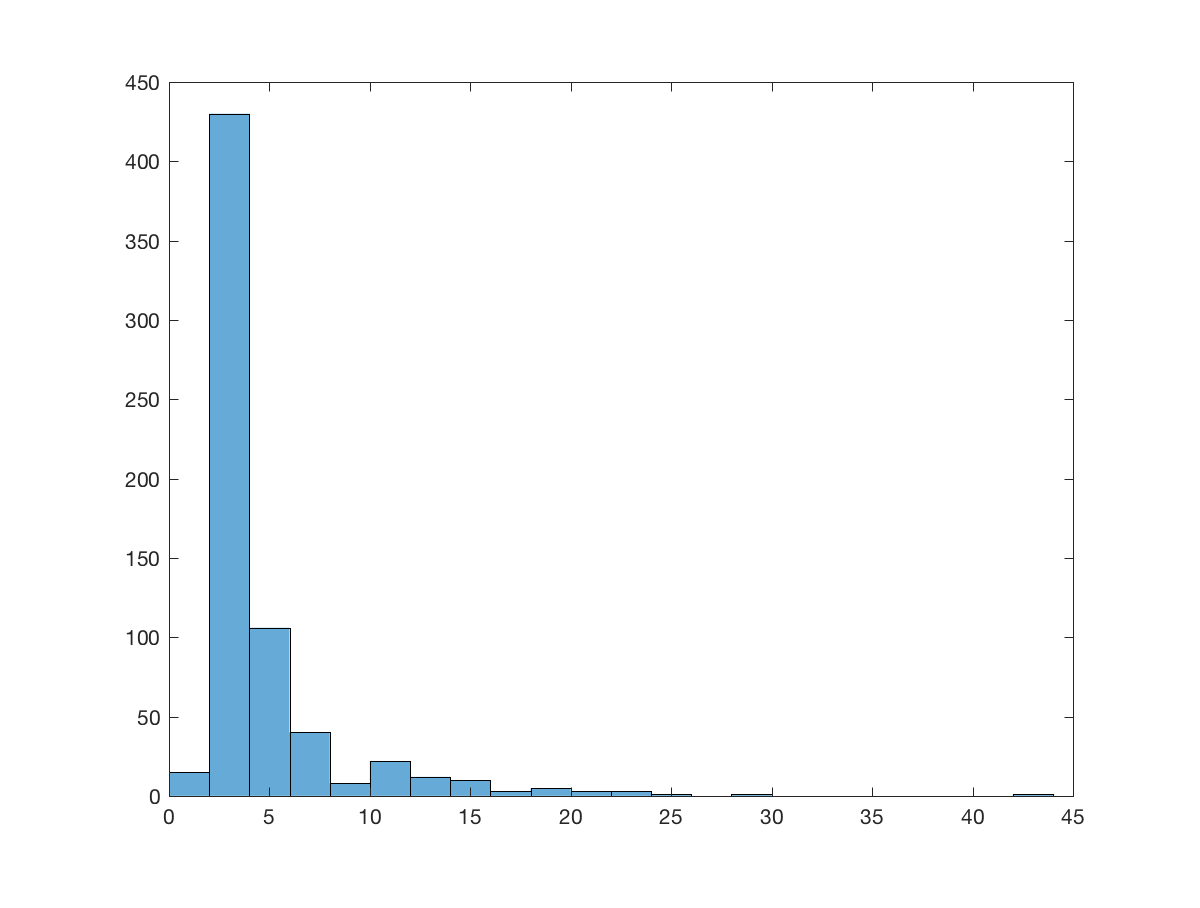
\includegraphics[width=.49 \textwidth]{Figures/AMp_Time_Lag_Histogram.eps}
%\caption{$AM_p$ curves on the left and a histogram of the time lags on the right.}
%\end{figure}
%
%\subsection{Radius Time Lag}
%
%\begin{figure}[h]
%\centering
%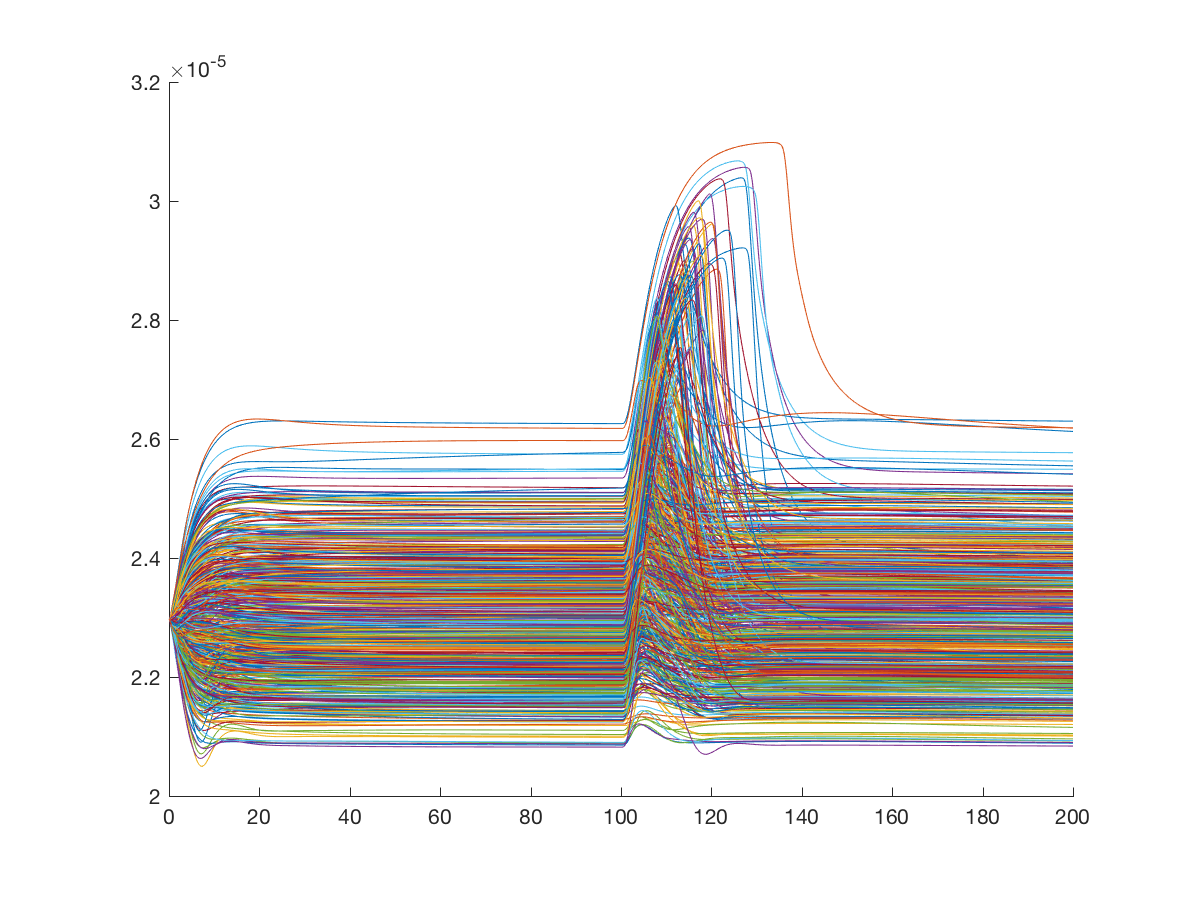
\includegraphics[width=.49 \textwidth]{Figures/Radius_Curves.eps}
%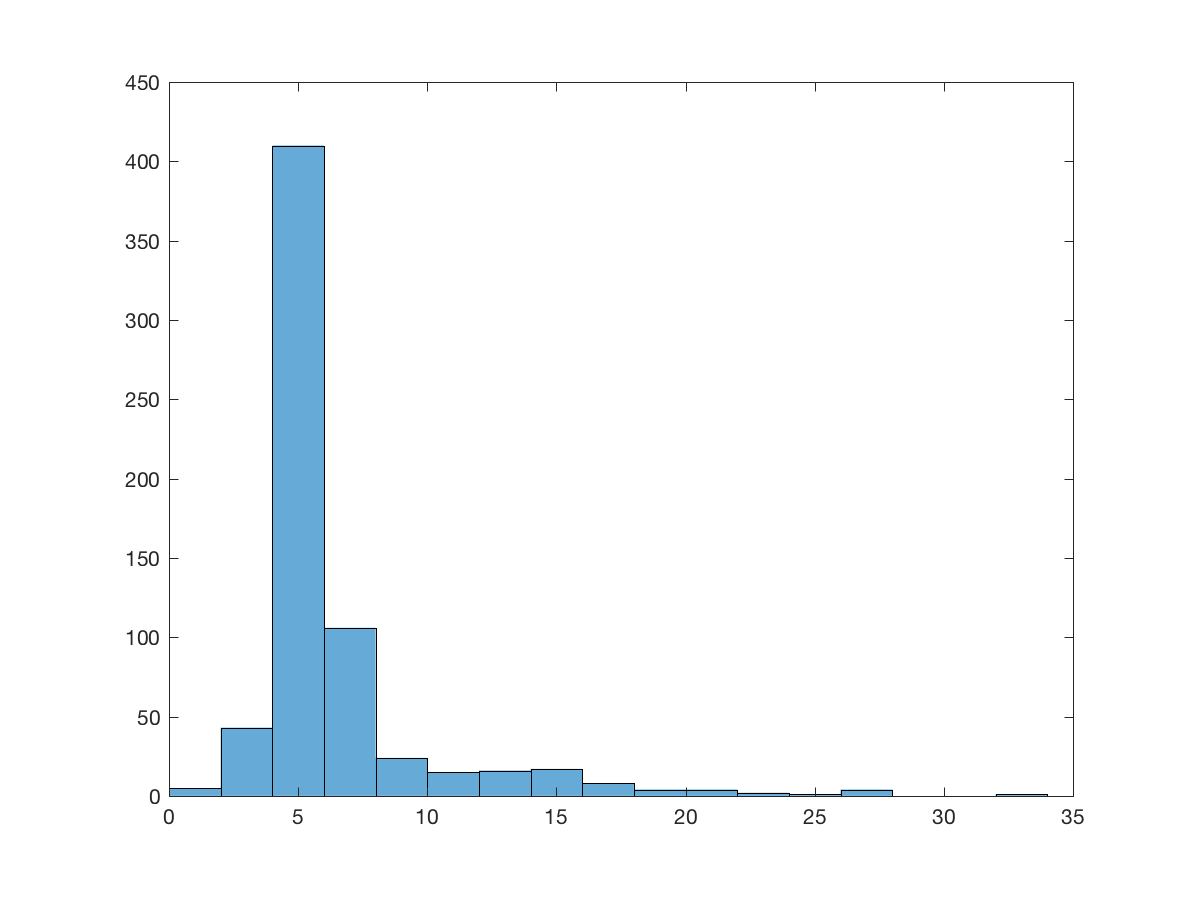
\includegraphics[width=.49 \textwidth]{Figures/Radius_Time_Lag_Histogram.eps}
%\caption{Radius curves on the left and a histogram of the time lags on the right.}
%\end{figure}


\section{Discussion}
ADD A DISCUSSION OF THE RESULTS IN TERMS OF THEIR PHYSIOLOGICAL INTERPRETATION

\section{Conclusion}
 A three stage methodology is presented for global sensitivity analysis of numerical cell models with a large number of parameters. To the authors knowledge, this is the first type of analysis which investigates neuroscience models of such size. The analysis investigated three quantities of interest pertaining to a numerical model of neurovascular coupling. The results indicated several prevalent features of the model. A significant influence of the persistent $Na^+$ channel activation variable on the average extracellular space $K^+$, a two parameter set (the inwardly rectifying $K^+$ channel shift parameter and the index for the cytosolic $Ca^{2+}$) which characterizes most of the variability in the average volumetric flow rate, and strong similarities between the most influential parameters for the average volumetric flow rate and minimum value of the combined actin/myocin complex.
 
In addition to the results reported in this article, four other QoI's were considered. Two of them, the maximum and average potassium concentration in the Astrocyte, were omitted because the parameter to QoI mapping is nearly constant and hence global sensitivity analysis is not necessary. Specifically, the mean of the QoI is approximately 37 times larger than its standard deviation for both cases. The other two unreported QoIs correspond to lag times. The first being the duration of time between the application of the stimulus and the minimum of the phosphorylated actin myosin complex, and the second being the duration of time between the application of the stimulus and the maximum of the radius. In both cases, the QoI exhibited highly nonlinear behavior which we were unable to approximate with linear or PC surrogates trained on the existing data. In fact, fitting such nonlinearities would likely require more samples than is computationally feasible for this model. The linear surrogate had 59\% and 47\% relative $L^2$ errors for these two QoIs, respectively. Our global sensitivity analysis methodology was unsuccessful because the linear surrogate was an unreliable tool for screening. Defining the QoI as the maximum/minimum value instead of the time lag makes the analysis more tractable. These maximum/minimum value QoIs were also considered and yielded similar results to the QoIs reported in the article.

For a given model and collection of samples, the methodology presented in this article may be applicable for some QoIs and intractable for others. The success of our method depends upon the surrogate models being sufficiently accurate. A general principle is that QoIs defined as averages will be more amenable for analysis than, for instance, minimum values or lag times. A practical benefit of our method is that any QoI may be considered without requiring additional model evaluations. The sampling and ODE solves are executed once, followed by computing the QoIs and performing global sensitivity analysis, which may be easily repeated for many different QoIs.
 
 
% Results showed that for the QoI defined by the average value of extracellular space $K^+$, the persistent $Na^+$  channel activation variable provided an approximately combined  62 \% of the variation in $K^+$ whilst the $K^+$ leak channel provided 21 \% and the KDR channel 11 \%. The dendrite length although in the first 5 ranked parameters provided only 3 \% variation. All other parameters were considered unimportant. \\
% For the second QoI (average value of the volumetric flow rate), the main variability ( 46 \%) was determined by the inwardly rectifying $K^+$ channel parameter which shifs the channel conductance to the right, whilst the index for the cytosolic $Ca^{2+}$ provided an approximately 33 \% influence. Three other parameters provided only a small influence but were associated with either the $K_{IR}$  or the BK $K^+$ channel conductances. 
% Finally the third QoI concerned the minimum value of the combined actin/myocin complex. In a related fashion to the volumetric flow rate, similar influential parameters appeared in the ranked list, the only two non-repeating parameters between the flow rate QoI and the actin/myson complex was the leak conductance GKi and $z_3$, which, as noted above, have very little effect. \\
% We should point out some limitations of the methodology in that other QoIs proved difficult if not impossible to analyse due to the resulting skewed distribution functions of the QoIs. Future work will investigate other methods which alleviate this difficulty. 
% It is important to note that the analysis itself is not one from which a more simple model of neurovascular coupling should be derived. In fact because different functions of the system are determined by a number of pathways (some of them independent) the numerical model in and of itself cannot be reduced to a mathematically analysable form. Indeed to investigate neurophysiological problems both from pathological and "normal" states models will very probably need to gain in complexity. The sensitivity analysis presented here however provides a searchlight on important and influential aspects of the model and hence the physiology. \\
% Attention should now be drawn towards how one can characterise which QoIs can in fact be analysed. 
%victory dance because we are the first people to do this type of problem.
%
% Forward looking paragraph, maybe multiscale modelling. 
%
%
%Look at other QoIs mention the fact that things don't work for every QoI future work how far can we push. How to characterise which QoIs we can deal with. 

\bibliographystyle{KathisBibstyle} % no .sty!
\bibliography{library}

\end{document}